\documentclass[11pt, a4paper]{report}

\usepackage{glossaries}
\loadglsentries{Glossary}
\makeglossaries

\usepackage{etoolbox}
\patchcmd{\chapter}{\thispagestyle{plain}}{\thispagestyle{fancy}}{}{}
\renewcommand{\thesection}{\arabic{section}}

\usepackage[utf8]{inputenc}
\usepackage[dvipsnames]{xcolor}

\usepackage{txfonts}
\usepackage{pdflscape}
\usepackage{todonotes}
\usepackage{float}

\usepackage{titlesec}
\titleformat{\chapter}[frame]{}{\thechapter}{0pt}{}
\titlespacing*{\chapter}{0cm}{-\topskip}{0pt}[0pt]
\titleformat{\chapter}{\normalfont\huge\bf}{\thechapter.}{20pt}{\huge\bf}

\setcounter{secnumdepth}{4}

\titleformat{\paragraph}
{\normalfont\normalsize\bfseries}{\theparagraph}{1em}{}
\titlespacing*{\paragraph}
{0pt}{3.25ex plus 1ex minus .2ex}{1.5ex plus .2ex}

\usepackage{graphicx}
\usepackage[english]{babel}
\graphicspath{ {images/} }
\usepackage{amsmath}
\usepackage{subscript} 
\usepackage{enumitem}
\usepackage{subfig}

\usepackage{mathtools}
\usepackage{amsmath}

\usepackage{listings}
\usepackage{booktabs}

\usepackage{booktabs}

\usepackage{fancyhdr}
\pagestyle{fancy}
\lhead{\hspace*{-0.7cm}
\includegraphics[width=7cm]{fhnw}}
\rhead{}

\usepackage{tabularx}
\newcolumntype{L}[1]{>{\raggedright\arraybackslash}p{#1}}

\usepackage{parskip}

\usepackage[round]{natbib}
\bibliographystyle{plainnat}

\usepackage{color}

\newcommand*{\Signatures}[2]{%
	\par\noindent\makebox[1.5in]{Location, Date, Signature}
	\hfill\makebox[1.5in]{Location, Date, Signature}
	\hfill\makebox[0.5in]{}%
	\vspace{0.7in}
	\par\noindent\makebox[1.5in]{\hrulefill}
	\hfill\makebox[1.5in]{\hrulefill}
	\hfill\makebox[0.5in]{}%
	\par\noindent\makebox[1.5in][l]{#1}      \hfill\makebox[1.5in][l]{#2}
	\hfill\makebox[0.5in]{}%
}%

\lstset{
basicstyle=\scriptsize\sffamily\color{black},
frame=single,
numbers=left,
numbersep=5pt,
numberstyle=\tiny\color{gray},
showspaces=false,
showstringspaces=false,
tabsize=1
}

\lstdefinelanguage{Kotlin}{
  keywords={package, as, typealias, this, super, val, var, fun, for, null, true, false, is, in, throw, return, break, continue, object, if, try, else, while, do, when, yield, typeof, yield, typeof, class, interface, enum, object, override, public, private, get, set, import, abstract, },
  keywordstyle=\color{NavyBlue}\bfseries,
  ndkeywords={@Deprecated, Iterable, Int, Integer, Float, Double, String, Runnable, dynamic},
  ndkeywordstyle=\color{BurntOrange}\bfseries,
  emph={println, return@, forEach,},
  emphstyle={\color{OrangeRed}},
  identifierstyle=\color{black},
  sensitive=true,
  commentstyle=\color{gray}\ttfamily,
  comment=[l]{//},
  morecomment=[s]{/*}{*/},
  stringstyle=\color{ForestGreen}\ttfamily,
  morestring=[b]",
  morestring=[s]{"""*}{*"""},
}

\lstdefinelanguage{XML}
{
  morestring=[b]",
  morestring=[s]{>}{<},
  morecomment=[s]{<?}{?>},
  stringstyle=\color{ForestGreen},
  identifierstyle=\color{NavyBlue},
  keywordstyle=\color{OrangeRed},
  morekeywords={xmlns,version,type,onAction,text,orientation}
}

\begin{document}
	\title{\textbf{Bachelor Thesis \\ - \\Automatic analysis and simplification of architectural floor plans}}
	\author{
			\begin{tabular}{l  l}
				Principals: & PlanFabrik GmbH \\
				Authors: & Alexander Wyss, Florian Bruggisser \\
				Supervising Prof.: & Prof. Dr. Simon Schubiger, Prof. Dr. Stefan Arisona \\ University: & FHNW Technik \\
				Email: & alexander.wyss@students.fhnw.ch \\ & florian.bruggisser@students.fhnw.ch				
			\end{tabular}
	}
	
\maketitle

\section{Abstract}

\tableofcontents
	
\section{Introduction}
\label{sub:Introduction}
\subsection{Starting position}
The company PlanFabrik GmbH creates floor plans for house technology. In a first
step, the plans are analysed and enhanced through an employee. He adds more
information to the plan, like room polygons or he marks areas, where house technology
can be installed and where not. Those areas are defined by different features. For example, usually the area close to windows has a higher density of pipes, emitting heat to the room. This is to compensate the heat loss that usually occurs on windows.
\\
The process of drawing those areas is currently tool supported, but still takes a lot of time, equal to the rising amount of rooms the employee has to analyze. The idea is to create a more automated system, which does require only a small amount of user input.

\subsection{Problem description}
\label{sub:ProblemDescription}
It takes the user a lot of time to manually create all the room-areas. This is due to the fact that he has to click every corner of each room to create a room-enclosing polygon. The fact that the current tool is not very precise, which means that errors in selecting the exact corner occur regularly. The user then has to rearrange the created corner, to fit the exact corner in the image. This process of selecting all the corners by hand is highly inefficient, especially for floor plans that have several hundred or even thousands of corners in it.
\\
An automated solution would provide a faster and more comfortable solution for the client. Additionally, the software may provide additional information that is needed. It can calculate the size of each room directly, which would otherwise have to be calculated by hand.

\subsection{Goals}
The idea of theory of this bachelor thesis is to compare different algorithms, which can automatically analyse floor plans and draw the polygons for the rooms. The goal in the end is to show and explain a way to solve the problem and decide which algorithms are used best. All of this will help us create a software that can do the automated analysis for basic floor plans. More complicated floor plans may hold problems that our algorithms can not find, those are supposed to be solved manually within an editor.
\\
In the end, the program is supposed to create an output-file with the information of the areas found, which is exportable to the existing software that currently handles the following processes.

\subsection{State of the art}
This section will explain how the current process for room recognition work at the Planfabrik GmbH. It will show the actual process that is to be replaced by the software described in this work. In an additional section, there will be a description of papers similar to this one. The idea is to show what solutions are already implemented which solve the problem. It also describes the work that was the foundation for our work.

\subsubsection{Manual process}
 The process for room and zone detection is done by hand. To start, they have an unprocessed architectural floor plan in a DWG or DXF format. It is processed by the \gls{gloss:CAD}. When defining the room size, the person processing the plan has to select the edge selection tool to create the room polygon. As a room has at least three corners, this process will take at least three mouse clicks for every room. This selection tool has its difficulties, as the person operating might not select the exact corner or miss-click, which leads to the loss of the whole selected polygon. From what we have experienced, every 8-16 corners there is going to be such an inaccuracy.
 
 To define the zones for different density of heating pipes, the same process of selecting a polygon is done. Depending on the elements of the plan, this can double the amount of user interactions. Some rooms might not contain those zones but others might have several.
 
 As a result the \gls{gloss:CAD} can calculate all the different sizes of the rooms.
 
\subsubsection{Similar works}
\label{sub:SimilarWorks}
This section introduces two papers \textit{A System to Detect Rooms in Architectural Floor Plan Images} \citep{mace_valveny_loctea_tabbone_2010} and \textit{Automatic Room Detection and Room Labeling from Architectural Floor Plans} \citep{ahmed_liwicki_weber_dengel_2012} which are two very recent paper on the exact problem of room segmentation. 

The second paper, written by Ahmed, Liwicki,Weber and Dengel, proposes a general structure for detecting floor plans. This structure will help us separate and compare the steps of the algorithms proposed in both of the discussed papers. It will also be used for the further structure of this document. They propose to separate the algorithm in three parts: \textit{Information segmentation}, \textit{Structural analysis} and \textit{Semantic analysis}. The information segmentation part contains all algorithms separating information (text, line thickness, symbols, etc.). The structural analysis contains algorithms that combine the important information from previous algorithms and and create a basic wall image. Finally the semantic analysis finds symbols and rooms based on information from the structural analysis.

The paper written by Mace, Valveny, Loctea and Tabbone uses several algorithms for information segmentation. They do a graphic/text separation because not all floor plan contain text. Therefore text like room names can not be used and have to be removed. Additionally they use a thick/thin line separation algorithm to separate the walls from the other lines of the floor plan. The walls are expected to be the thickest lines on the plan.

For structural analysis they use the hough transformation, which is described in Section \ref{subsubsec:Hough transformation}, in combination with image vectorization. This is used for a simple wall detection algorithm. The wall detection works on an image of the contour of the walls. They take two lines that are close together and have the same orientation and check if the pixels in between those lines are black. If so this is an actual wall due to the fact that before taking the contour of the walls they were connected. 

The room detection in the semantic analysis is done with a polygon partitioning technique, that uses the wall as a convex hull and tries to split it up in smaller polygons (rooms), that all have to be convex. This, in combination with the fact that rooms are mostly rectangular shape, which is adjusted during post-processing, will detect the rooms.

\begin{figure}[H]
	\centering
	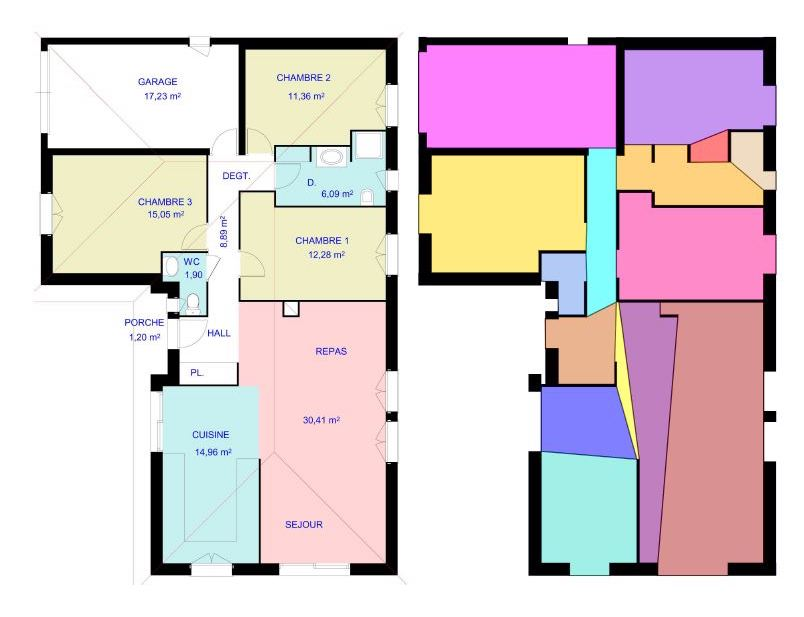
\includegraphics[width=1.0\textwidth]{paper1_floorplan}
	\caption{Room segmentation with the algorithm used in \textit{A System to Detect Rooms in Architectural Floor Plan Images} by Mace, Valveny, Loctea and Tabbone. }
	\label{fig:paper1_floorplan}
\end{figure}

The second paper mentioned above by Ahmed, Liwicki, Weber and Dengel, takes a similar approach. For information segmentation they also separate text/lines as well as separate thick/thin lines. The difference is that they use the text to name the rooms. Additionally they separate the image in thick, medium and thin lines instead of just thick and thin. Thick lines represent external, medium internal walls and thin lines represent symbols.

For structural analysis they also use a similar approach for wall detection but additionally close additional gaps with a convex/concave hypothesis, further described in the paper. Those algorithms lead to a very refined image of the walls, with better results than proposed in the previous paper.

For the semantic analysis they use \gls{gloss:SURF} as a algorithm to detect doors. This helps separating rooms, because the the definition of separation is, that there has to be a door connecting them. To find the rooms, a connected component analysis is used on the wall image. Gaps where a doors should exist, are closed with \gls{gloss:SURF} and therefore rooms are defined by a connected component. Each of these rooms will then be labeled with a name from the text layer, that overlap into the area of the detected room.

\begin{figure}[H]
	\centering
	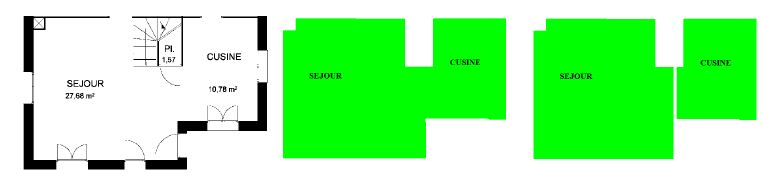
\includegraphics[width=1.0\textwidth]{paper2_floorplan}
	\caption{Room segmentation with the algorithm used in \textit{Automatic Room Detection and Room Labeling from Architectural Floor Plans} by Ahmed, Liwicki, Weber and Dengel. }
	\label{fig:paper2_floorplan}
\end{figure}

Both of those papers have a room detection rate between 80-90\%. The important part though is the room recognition rate which is only around 50\% for the work by Mace, Valveny, Loctea and Tabbone. This is really low for a real world use-case. The work by Ahmed, Liwicki, Weber and Dengel improves this rate up to about 80\%, which is a big improvement. This is most likely due to the fact that they use \gls{gloss:SURF} as a door recognition algorithm, which helps separating the rooms more accurately. Both works struggle with the difference, in how symbols and walls are depicted in architectural floor plans. They can only detect those rooms, if the walls are the thickest lines on a plan and there is no interference from symbols.
 

\subsection{Metrics}
To have a measurement, to compare our product to what is already in place at the Planfabrik GmbH, we went there and collected two values. Those values are the time which is needed to do the room segmentation and how many mouse-clicks it would take. We did that on five different floor plans, that were preselected by us. They were selected after the difficulty to analyse, rated by ourself, as well as their difference in the number of rooms.

The plans chosen are the following:

AN\_1
50er
A1\_OG



The time was taken with a countdown clock on an iPhone and was stopped manually by hand. This led to a time deviation of usually 1-2 seconds longer than the actual time. The same will be done for our tests, so that this difference will not matter. The clicks made were counted by hand.
An estimate of how many clicks are made on a floor plan, is made along the following rules. For every room it usually takes the amount of edges the room has, plus two additional clicks to create and confirm the room. There are also some additional clicks at the beginning, to start the selection as well as the end to confirm and save it.
What was not taken into consideration in these tests are miss-clicks. These occur quite often. There are two different types of errors that follows from these. Either the last selected edge was way off and has to be corrected, which will take 3 additional clicks. Or it deletes all the work done by now and all rooms have to be reselected. During our tests, this second error happened twice, during six test-runs. That the edge selection is not correct happens around every third or fourth room. All together it can generate an additional 10 percent of clicks over an several floor plans.

\begin{table}[H]
	\centering
	\begin{tabular}{@{}lll@{}}
		\toprule
		Plan          & Clicks & Time (S) \\ \midrule
		AN\_1         & 77     & 182 \\
		50er          & 85     & 170  \\
		A\_1OG        & 222    & 452 \\ \bottomrule
	\end{tabular}
\caption{Time and clicks used to detect the all the rooms. These times were done with the program used at the Planfabrik GmbH for the images shown. }
\end{table}

This table shows the test results for all the different floor plans. With this data, we will make comparisons in the \textit{Implementation} (Section~\ref{sub:Implemenation}) to test how effective our product is compared to the one in use.

Based on information from the Planfabrik GmbH, each hour of work costs them 80 CHF. Therefore any time saved on those room selections saves them a considerable amount of money. This is why the time measurement takes an important part in our metrics. Additionally any time the algorithm is running and the worker can focus on other things will not count towards the time taken for room recognition. This may also be and advantage of this project, due to the fact that its an automated algorithm and the worker can focus on other work, till the algorithm has finished.

\subsubsection{Object detection perfomance}
\label{sub:ObjectDetectionPerfomance}

To measure the performance of the object detection, we calculate the precision and recall of the different algorithm results (Figure~\ref{fig:PrecisionAndRecall}). Both scores together give us a comparable metric, called F1 score \citep{sokolova_lapalme_2009}.

\begin{figure}[H]
	\centering
	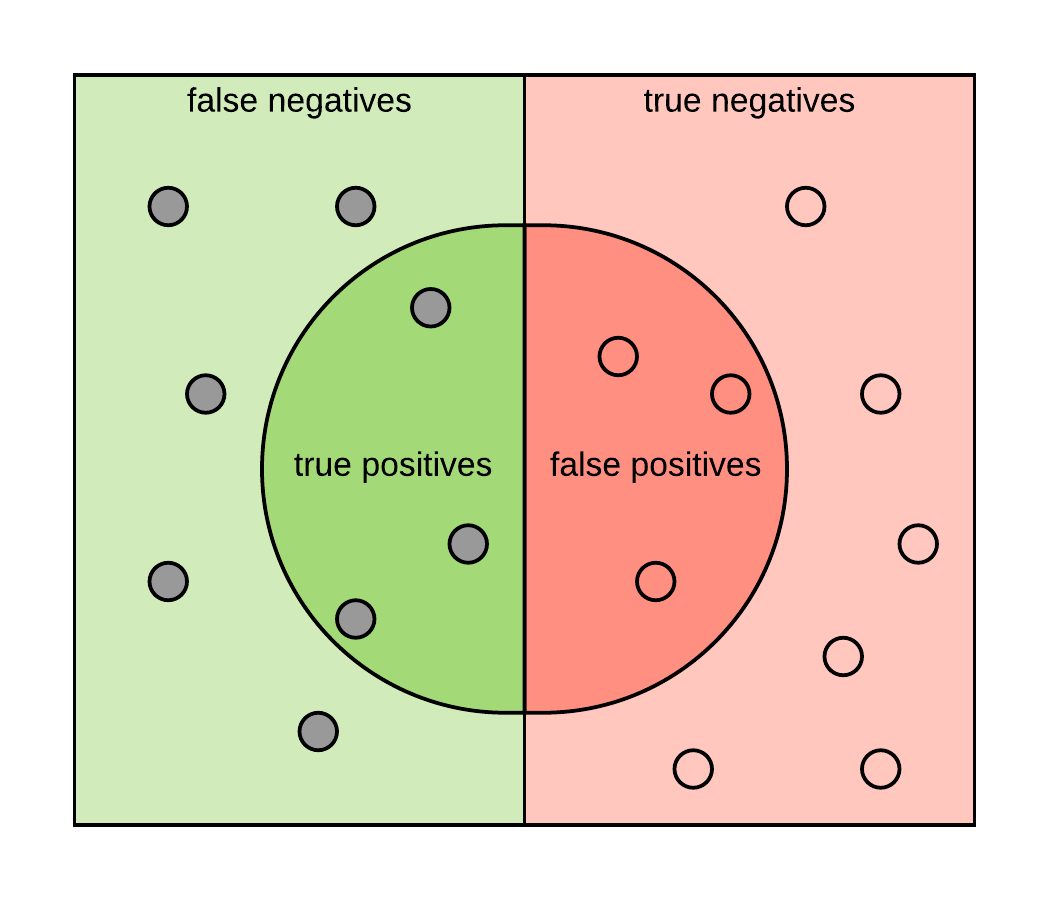
\includegraphics[width=0.7\textwidth]{PrecisionAndRecall}
	\caption{Precision and Recall visualisation. On the left side are the relevant elements.}
	\label{fig:PrecisionAndRecall}
\end{figure}

The reason to use precision and recall is, that both together create an accurate tool to measure the accuracy of an object detection algorithm. For further explanation of the used metrics, we use the abbreviation of the following terms:

\begin{enumerate}[label=]
    \item \textit{TP}: true positives
    \item \textit{FP}: false positives
    \item \textit{TN}: true negatives
    \item \textit{FN}: false negatives
\end{enumerate}

\paragraph{Precision}
\label{sub:Precision}

The precision score takes \textit{TP} and all retrieved documents (\textit{TP} and \textit{FP}), to calculate a score, which reflects the normalised amount of how many selected elements are relevant (Equation~\ref{eq:Precision}).

\begin{equation} \label{eq:Precision}
\begin{gathered}
precision = \frac{TP}{TP \cup  FP}
\end{gathered}
\end{equation}

\paragraph{Recall}
\label{sub:recall}

The recall score takes \textit{TP} and all positive documents (\textit{TP} and \textit{TN}), to calculate a score, which reflects the normalised amount of how many relevant elements are selected (Equation~\ref{eq:Recall}).

\begin{equation} \label{eq:Recall}
\begin{gathered}
recall = \frac{TP}{TP \cup  TN}
\end{gathered}
\end{equation}

\paragraph{F1 Score}
\label{sub:F1Score}
The \textit{F1} score combines the precision and recall with the harmonic mean (Equation~\ref{eq:F1Score}).

\begin{equation} \label{eq:F1Score}
\begin{gathered}
F_{1} = 2 * \frac{precision * recall}{precision + recall}
\end{gathered}
\end{equation}


\section{Software Architecture}
This chapter describes the solution developed during our work. At the beginning the software architecture will be explained, followed by the partial steps and experiments which were needed to find the solution.
\\\\
The software architecture has to fulfil multiple requirements for this project. It should be easily extendable with new algorithms and ui extensions. The input and output format of the application should be independent from the algorithms to support different file types like bitmap images or \gls{gloss:DXF}/\gls{gloss:DWG} formats. The algorithms of the application should be link together as workflows which then can be executed by an engine in parallel.

\begin{figure}[h]
  \centering
      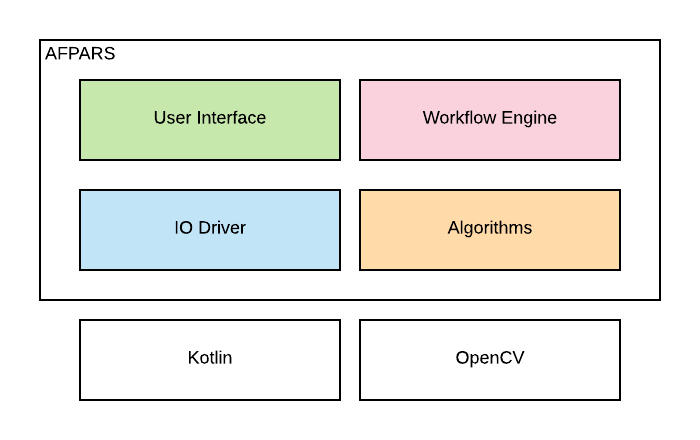
\includegraphics[width=1\textwidth]{AFPARS_Architecture}
  \caption{AFPARS software architecture.}
  \label{fig:AFPARS_Architecture}
\end{figure}


To fulfil these requirements, the architecture of the software is split into four parts as shown in Figure \ref{fig:AFPARS_Architecture}. The complete application is based on the \acrfull{acro:JVM} where \gls{gloss:Kotlin} is running on. For image processing and recognition the application uses the library \gls{gloss:OpenCV}.

\todo{What else should I write?}

\pagebreak

\subsection{Input / Output}
To support the different input and output formats the architecture uses a meta format for the
floor plan images called AFImage. Different drivers add the support for multiple file formats. With this architecture it is possible to extend the software with new file formats and work internally with the meta container.

\begin{figure}[h]
  \centering
      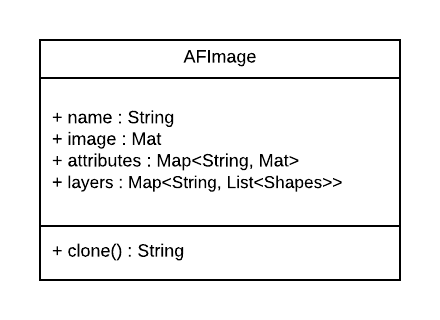
\includegraphics[width=0.6\textwidth]{AFImage_CD}
  \caption{AFImage class diagram.}
  \label{fig:AFImage_CD}
\end{figure}

The meta container AFImage contains multiple attributes (see Figure \ref{fig:AFImage_CD}) which can be used by algorithms to get information created by other algorithms or store information into an existing image.

\subsection{Algorithm}
\todo{rewrite, this is nonsense}
To reuse algorithms in different workflows, the software architecture splits the algorithms into small parts which then can be connected together to pipelines. The algorithm itself does not know in which context it is running. As input parameter it gets just an AFImage from the last algorithm output and is able to return an AFImage again (see Figure \ref{fig:IAlgorithm_CD}). 

\begin{figure}[h]
  \centering
      \includegraphics[width=0.6\textwidth]{IAlgorithm_CD}
  \caption{Algorithm interface class diagram.}
  \label{fig:IAlgorithm_CD}
\end{figure}

Because a lot of the algorithms need parameters to be set manually, there is the possibility to flag these parameters with an attribute in the code and the software is then able to automatically show a slider in the user interface. With this slider the user is able to set the parameter or use the default values (See Figure \ref{fig:parameter_window}).


\begin{figure}[h]
  \centering
      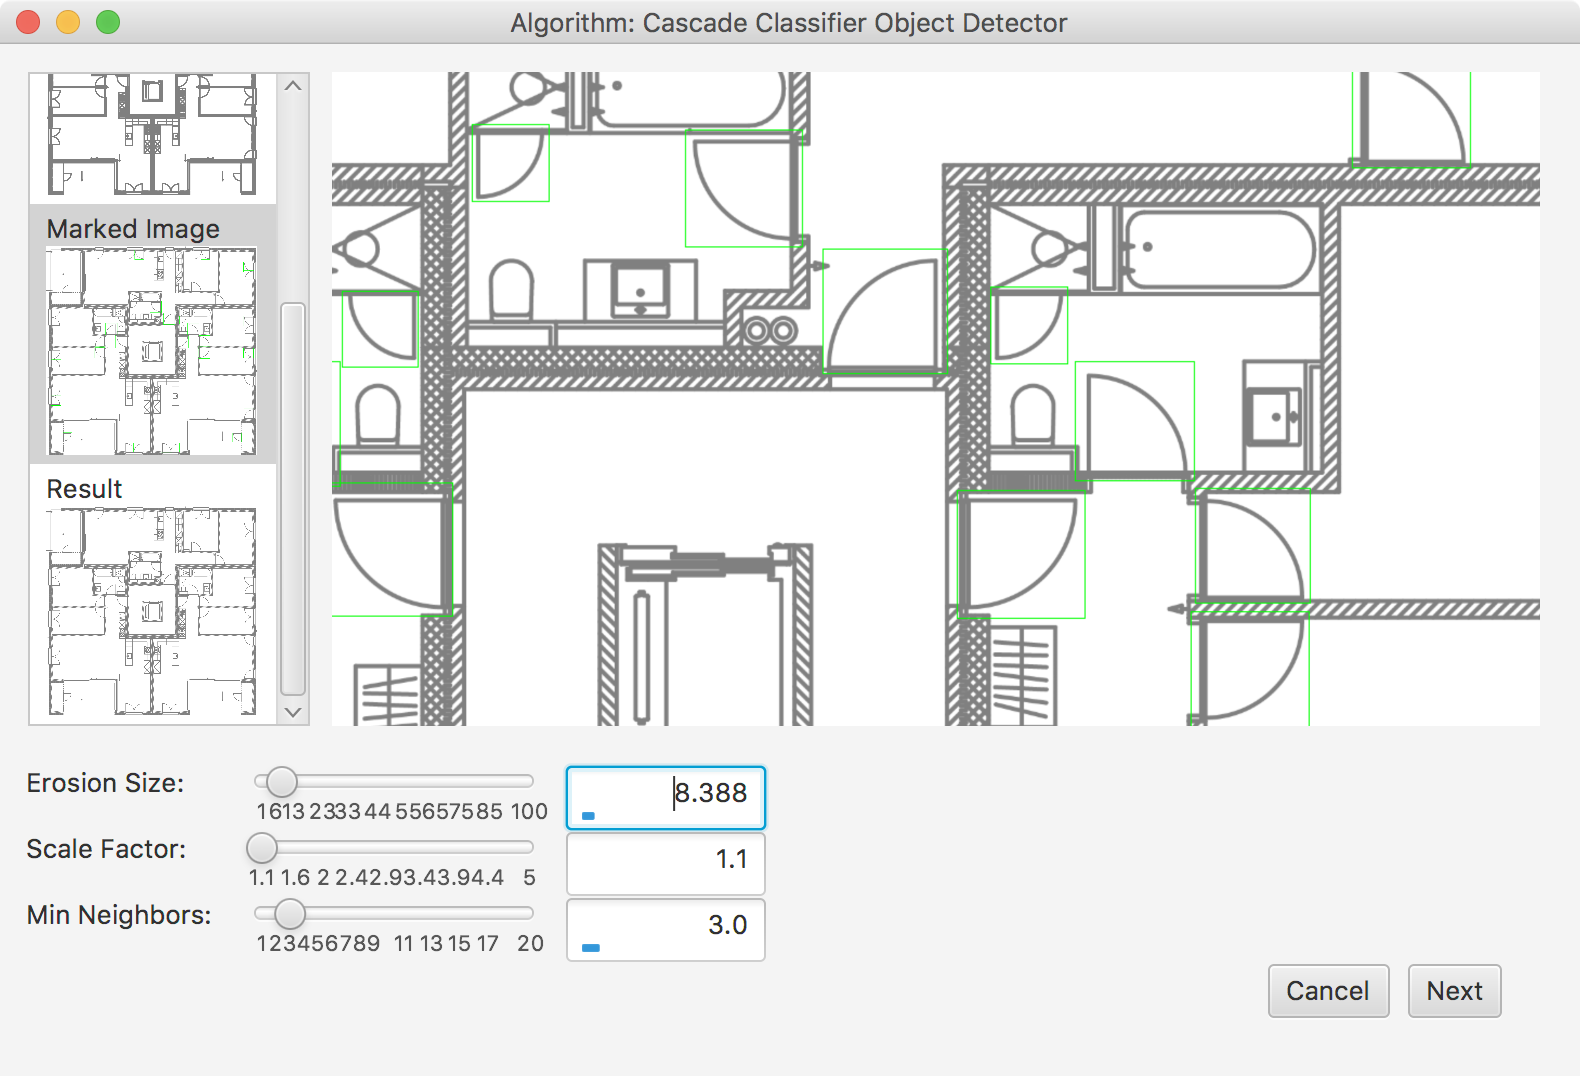
\includegraphics[width=0.6\textwidth]{parameter_window}
  \caption{Flag based parameter window.}
  \label{fig:parameter_window}
\end{figure}


\subsection{Workflow}

\begin{figure}[h]
  \centering
      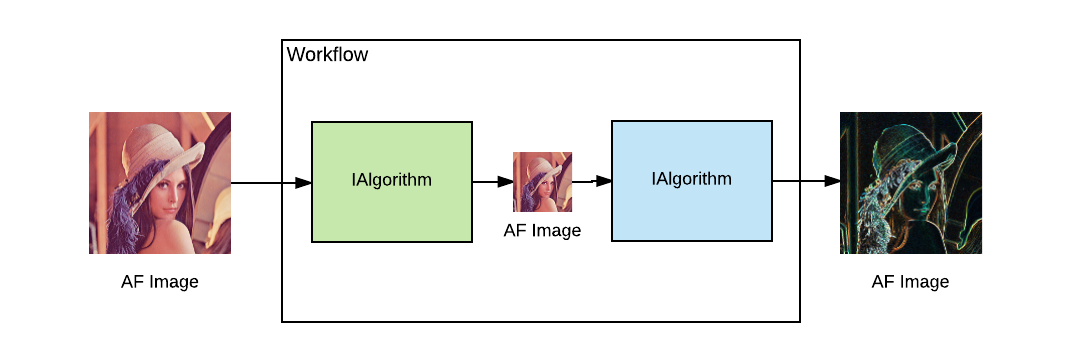
\includegraphics[width=1\textwidth]{workflow}
  \caption{Workflow example with two algorithms.}
  \label{fig:Workflow}
\end{figure}

\subsection{User Interface}
\missingfigure{User Interface Image.}
\todo{Why it looks like that. (Andere Software)}
\section{Implementation}
\subsection{Software Architecture}
\subsubsection{User Interface}
\subsubsection{Algorithm}
\subsubsection{Workflow}
\subsection{Analyse}
\subsubsection{Noise Removal}
\subsubsection{Room Detection}
\subsubsection{Object Detection}
\section{Theory}
\subsection{Information Segmentation}
\subsubsection{Erosion and Dilation}
\label{subsubsec:Erosion and Dilation}
In our project we need dilation to strengthen small features that we want to be highlighted as well as to get rid of small details in the picture itself. We use it in early preprocessing. It helps together with the erosion to clean up pictures to further process them without too many interfering objects in the image. The main usage is to extract an image that features all the walls and has as few as possible other lines on it \citep{burger_burge_2016}.

For our project we use the binary grayscale erosion~\eqref{eq:GrayscaleErosion}.
The erosion uses the following principle to work.


\begin{equation}\label{eq:GrayscaleErosion}A \ominus B = \{ z\in E | B \subseteq A \}\end{equation}  
\begin{equation}\label{eq:StructuringElement}where: B_{z} = \{b+z | b \in B\} with \forall z \in E \end{equation}

A is a binary image in the Euclidean space or an integer grid. The erosion is done with the structuring element B~\eqref{eq:StructuringElement} on the image A. The structuring element has to be a subset or equal to A, otherwise there will be no erosion. The mask B will be applied to all pixels possible, if the mask fits on the center pixel of A, the value will be retained. Otherwise it will get deleted. This means that only when B is completely contained in A, values of pixels are retained.

Binary dilation uses the exact same process. The only difference compared to the erosion is that the deletion of the pixel will not be setting pixel values to white 1, but to black 0. Both of those processes are inherently the same and can be summed up under the term morphological operation. These are altering the image with a mask, as we did here for erosion and dilation.

\subsubsection{Geodesic Dilation}
\label{subsubsec:GeodesicDilation}

Geodesic dilation is an iterative morphological transformation for the reconstruction of marked foreground objects. Instead of the normal dilation (Section~\ref{subsubsec:Erosion and Dilation}) it uses a marker image $F$ which defines the starting points of the dilation, a mask image $G$ which defines the constraints of the dilation and a structuring element $B$ which describes the dilation itself.

For example the algorithm is used to reconstruct the area of the brightest points of a distance transformed image (Section~\ref{subsubsec:Distance transformation}). We used this for extracting and enhancing the room center points which then are used as marker points of the watershed marker image (Section~\ref{subsub:watershed}).

The geodesic dilation is defined as $D_{G}^{(n)}(F)$ where n is the iteration size and $F$ the marker with respect to the mask $G$. As a precondition $F$ is a subset of (or is included in) $G$: $F \subseteq G$.

There is no implementation in \gls{gloss:OpenCV} of this algorithm. We implemented it ourself and give here short implementation overview.
	
\begin{equation} \label{eq:geodesic_dilation_iteration}
\begin{gathered}
D_{G}^{(0)}(F) = F
\\
D_{G}^{(1)}(F) = (F \oplus B) \cap G)
\\
D_{G}^{(n)}(F) = D_{G}^{(1)}(D_{G}^{(n-1)}(F))
\end{gathered}
\end{equation}

Where:
\begin{itemize}[label=]
    \item $F$: is the marker image
    \item $G$: is the mask image
    \item $B$: is the structuring element
    \item $n$: is the iteration index
\end{itemize}

As seen in equation~\eqref{eq:geodesic_dilation_iteration}, a geodesic dilation with zero iterations is equal to the initial marker image. In the first iteration the marker image $F$ is dilated with the structural element $B$ and the result of that dilation is intersect with the mask image. This intersection limits the dilation to the marker constraints. After one iteration the next iteration uses the result of the last iteration as new marker image $F$.

The iteration stops as soon as the the difference (absolute array norm) between $F^{n}$ and $F^{n-1}$ becomes less then $\epsilon$ which in our case is 0.0001.

\subsubsection{Distance transformation}
\label{subsubsec:Distance transformation}
The distance transformation is as well as the erosion and dilation a morphological operation. In our project it serves the purpose to find bassins for the watershed algorithm. This is used to define the foreground picture. We will explain this further in the wathershed discussion.
It is used after preprocessing to find the center of what is supposed to be rooms. This algorithm is only used in combination with the watershed.

The algorithm that openCV uses is called cvDistTransform and uses an euclidean distance to calculate the output image. The input for this transformation is a binary image $I(u,v) = I(x)$ which will be separated into a foreground \eqref{eq:Foreground} and background \eqref{eq:Background} image.
\begin{equation}\label{eq:Foreground}FG(I) = {x | I(x) = 1}\end{equation}
\begin{equation}\label{eq:Background}BG(I) = {x | I(x) = 0}\end{equation}
The formula for the distance transformation of $I$, $D(x)$ itself is defined as:
\[D(x) :=\min_{x' \in FG(I)} dist(x,x') \]
It applies to any pixel $x = (u,v)$ of the input image. If the pixel is part of the foreground image $FG(I)$ then the result of the transformation $D(x)$ is zero. As said above, the distance formula $dist(x,x')$ is the euclidean distance \eqref{eq:EuclideanDistance} (also called $L_{2}-Norm$) between two pixels.
\begin{equation}\label{eq:EuclideanDistance}dist(x,x') = ||x - x'|| = \sqrt{(u - u')^2 + (v - v')^2}\end{equation}

Since the exact calculation with the euclidean distance takes a lot of computational power openCV uses the Chamfer-Algorithm instead. This algorithm runs a two masks over the image. The first mask $M_{L}$ \eqref{eq:LeftMask} is run over in a diagonal manner over the image starting in the top left corner of the image. The second mask $M_{R}$ \eqref{eq:RightMask} does the same in reverse starting at the bottom right corner. Those masks are a matrix that represent the euclidean distance between the center and the pixels around it. Each mask only changes the pixels in the direction they are run through the image \citep{burger_burge_2016}. As a result, the masks look similar to the following ones:
\begin{equation}\label{eq:LeftMask} M_{L} = \begin{bmatrix} . & . & .\\ . & x & m_1 \\ m_2 & m_1 & m_2 \end{bmatrix}\end{equation}
\begin{equation}\label{eq:RightMask}M_{R} = \begin{bmatrix} m2 & m1 & m2 \\ m1 & x & . \\ . & . & . \end{bmatrix} \end{equation}

This all leads to the resulting effect shown in the image below \citep[Section 3.3.3]{szeliski_2011}.
\todo{Make image of distance transformation before and after}
Source: http://stackoverflow.com/questions/7426136/fastest-available-algorithm-for-distance-transform

\subsubsection{Find contours}
\label{sub:FindContoursTheory}
The find-contours algorithm was used several times during the implementation of this project for different uses. Those uses will are described in the "Implementation" part of this document. What the algorithm does is that it finds the borders or the contour of different components in an image. The algorithm used by OpenCv was first described by Suzuki and Abe \cite{suzuki_abe_1985}. This will be a short description of what the algorithm does as the algorithm itself is quite complicated and can be reviewed completly in their paper.

The algorithm searches for borders in an image. A border is for example on a binary image where the pixel value changes from 0 to 1 or the other way. The algorithm defines two components that are possible. There are borders, that is where the value changes. Then there are holes, these are the spaces between the borders as well as the background.

The algorithm searches on pixels on the image from the outside for borders. As soon as it meets a pixel that is part of a border it stops and assigns this border a uniquely identifiable number. This marks it as a border. Each found border will also be assigned a parent, this is the border that encloses this border. This will define a hierarchy of all borders. The algorithm then follows the detected border and sets all pixels that are part of it to the same number. This will be repeated until all pixels of the image are visited and all borders are found.

This is a very simplistic explanation of what the algorithm does. The whole algorithm is described and proved in the work of Suzuki and Abe \cite{suzuki_abe_1985} for anyone interested in the exact algorithm.

\begin{figure}[h]
	\centering
	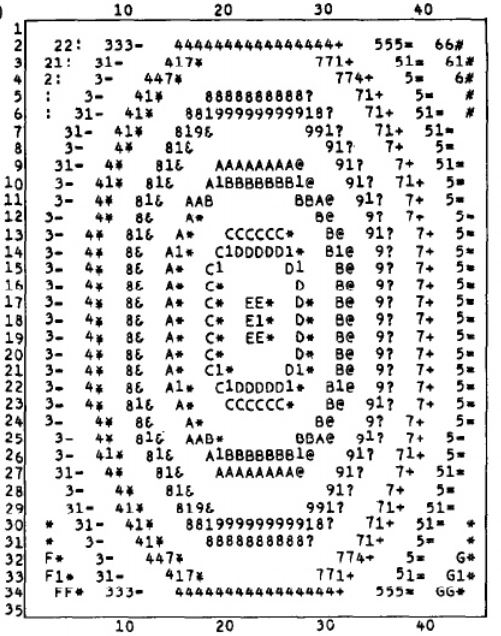
\includegraphics[width=0.4\textwidth]{suzuki_abe}
	\caption{The representation of borders in an example image in the paper of Suzuki and Abe. The value represent the different borders of connected pixels.}
	\label{suzuki_abe}
\end{figure}


\subsubsection{Harris corner detection}
\label{subsubsec:HarrisCornerDetection}
The corner detection algorithm is used to find corners in an image that contains mostly walls. Its purpose is to find the edges of all walls and therefore provide important information for the door gap closing algorithm. Why this information is needed will be explained in the section about this door gap closing algorithm.
This project uses the Harris corner algorithm due to its reliability, simplicity in implementation and the good results we got after the first uses. The algorithm itself is implemented by OpenCv.
The idea of the algorithm is that there are edges wherever the gradient of the image function is high for more than one direction.
First it calculates the basic partial derivatives of the image function $I_{x}(u,v)$ in horizontal and vertical direction. This is done for every position in the image $(u,v)$.
\begin{equation}A(u,v) = I_{x}^2(u,v)\end{equation}
\begin{equation}B(u,v) = I_{y}^2(u,v)\end{equation}
\begin{equation}C(u,v) = I_{x}^2(u,v) * I_{y}^2(u,v)\end{equation}

All of those elements will be part of a local structure matrix M.
\begin{equation}M = \begin{pmatrix} A & C \\ C & B \end{pmatrix}\end{equation}
Afterwards all three scalar fields will be smoothed with a linear Gaussian filter and be represented as a Matrix $\bar{M}$.
The two eigenvalues of the Matrix $\bar{M}$
\begin{equation}\lambda_{1,2} = \dfrac{trace(\bar{M})}{2} \pm \sqrt{(\dfrac{trace(\bar{M})}{2})^2 - det(\bar{M})} \end{equation}
are positive and contain important information about the local structure. In a area with no corners $\bar{M} = 0$  as well as the two eigenvalues $\lambda_1 = \lambda_2 = 0$. To find a corner there needs to be a strong edge in the main direction (bigger eigenvalue) as well as in the direction of its normal (smaller eigenvalue). 
To find the corner strength itself the Harris corner detection uses the function 
\begin{equation}Q(u,v) := det(\bar{M}(u,v)) - \alpha * (trace(\bar{M}(u,v)))^2\end{equation}
whereas the parameter $\alpha$ defines the sensitivity of the detector. A candidate for a corner is found when
$Q(u,v) > t_H$
with the threshold $t_{H}$ being around 10 000 to 1 000 000. To find the exact corner it finds groups of candidates that are close to each other are all eliminated but the best candidate.

\subsubsection{Point clustering}
\label{sec:PointClustering}
Due the fact, that the corner detection (Section~\ref{subsub:CornerDetection}) sometimes detects too many points at a wall corner, the aim of this algorithm is to create a sparse point group. This algorithm assigns a list of points into groups and combines them together to one single point, which represents the average position of all points in the group (Figure~\ref{fig:HCPointClustering}).

\begin{figure}[h!]
	\centering
	\subfloat[Multiple points at wall corner]{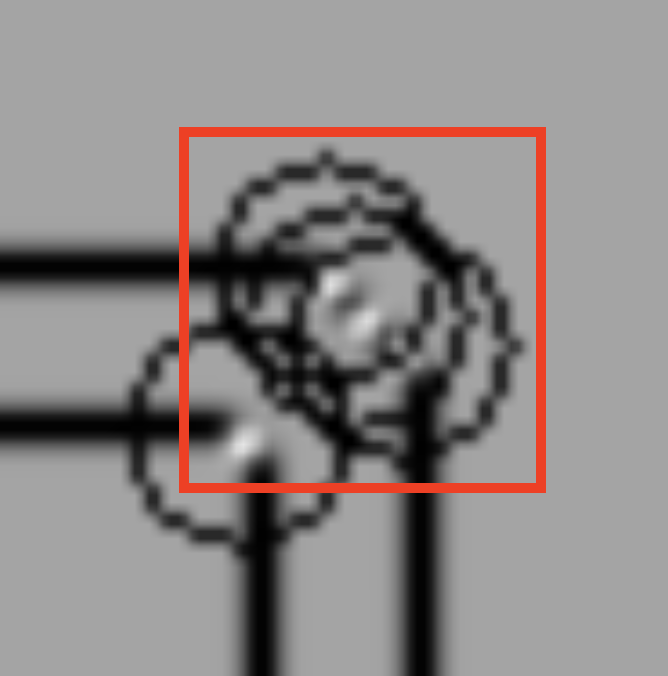
\includegraphics[width=0.4\textwidth]{hc_overdetection}\label{fig:hc_overdetection}}
	\hfill
	\subfloat[Averaged point at wall corner]{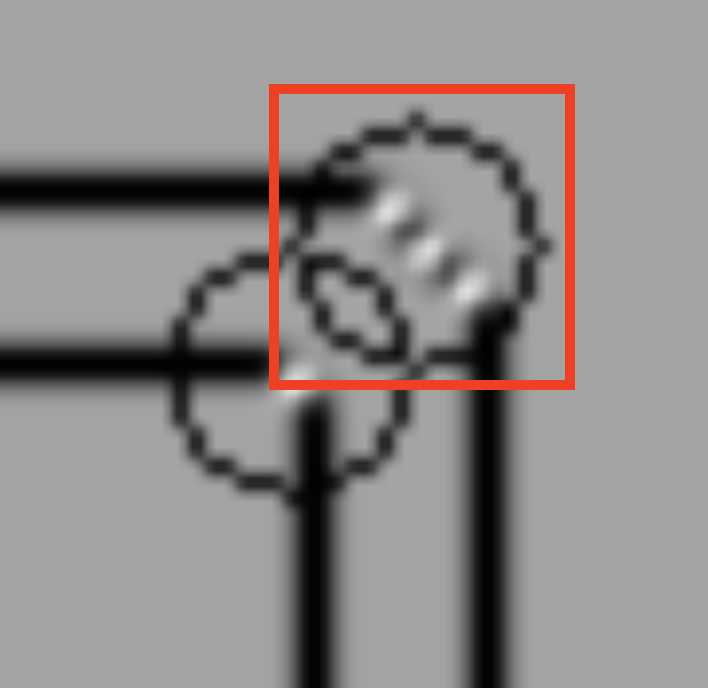
\includegraphics[width=0.4\textwidth]{clustered_hc_detection}\label{fig:clustered_hc_detection}}
	\caption{Harris Corner detection before point clustering (a) and after point clustering (b).}
	\label{fig:HCPointClustering}
\end{figure}

The algorithm takes a list of points $M$ in $R^2$ and a maximal distance $d$ as input and returns a list of grouped points. If the $L^2$ distance between two points, is less then the maximal distance $d$, the points are adjacent and assigned to the same group.

For each unprocessed point in the group, the algorithm is repeated to avoid a greedy behaviour of the algorithm.

A single point without any adjacent remains as it is (Figure~\ref{fig:point_clustering_single}). Multiple points are combined into one single point (Figure~\ref{fig:point_clustetring_multiple_close}). Sometimes it leads to large groups, because points which are not adjacent, can be assigned to the same group. In figure~\ref{fig:point_clustering_multiple_spread}, that case is visualised, where multiple points are assigned to the same group, which are further away then the maximal distance $d$.

\begin{figure}[h!]
	\centering
	\subfloat[Single point]{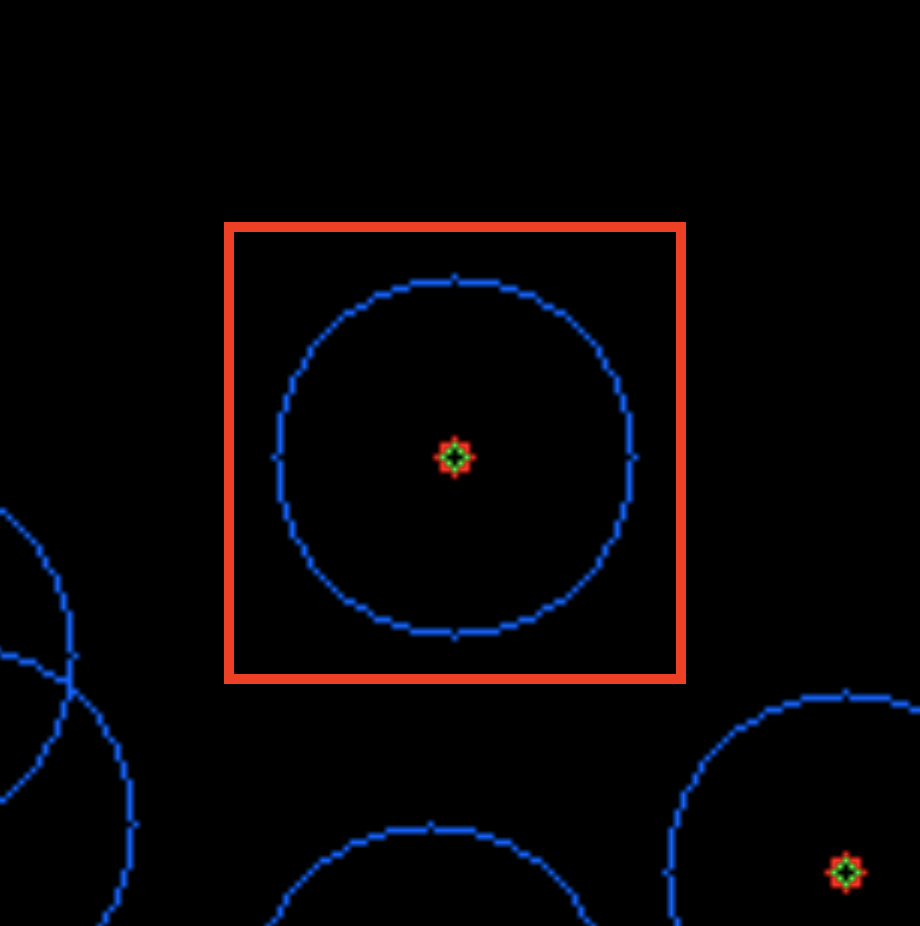
\includegraphics[width=0.3\textwidth]{point_clustering_single}\label{fig:point_clustering_single}}
	\hfill
	\subfloat[Multiple points]{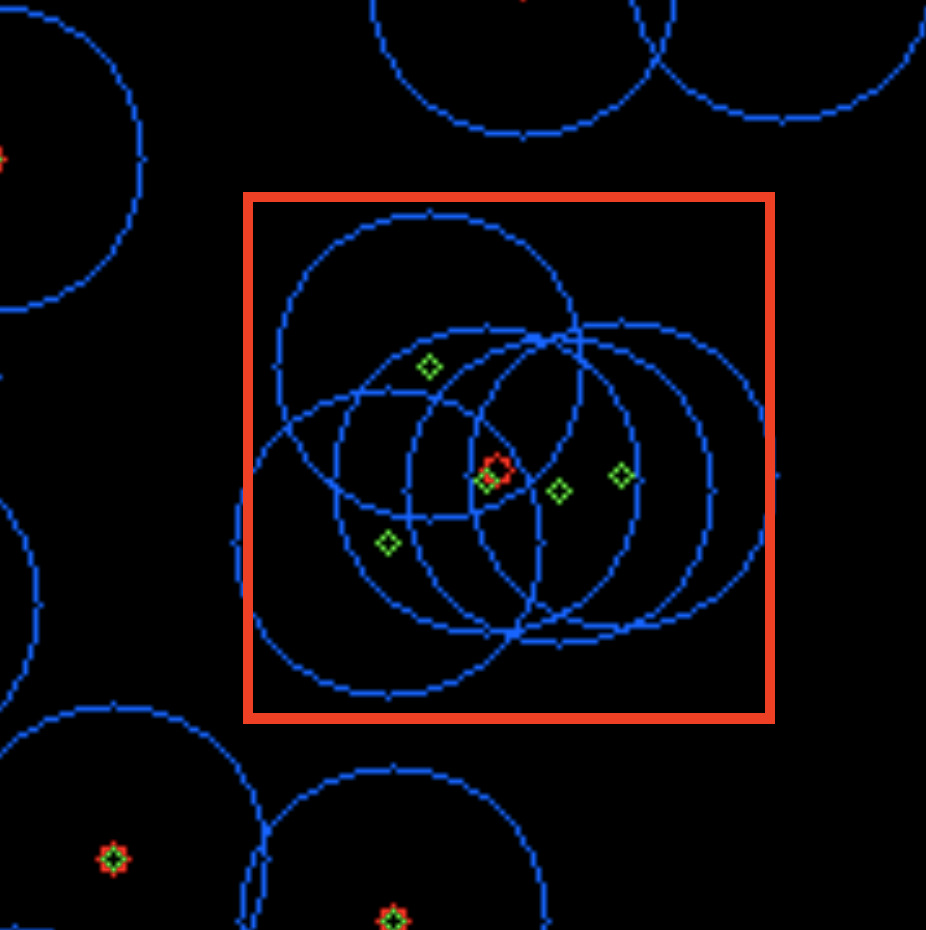
\includegraphics[width=0.3\textwidth]{point_clustetring_multiple_close}\label{fig:point_clustetring_multiple_close}}
	\hfill
	\subfloat[Multiple spread points]{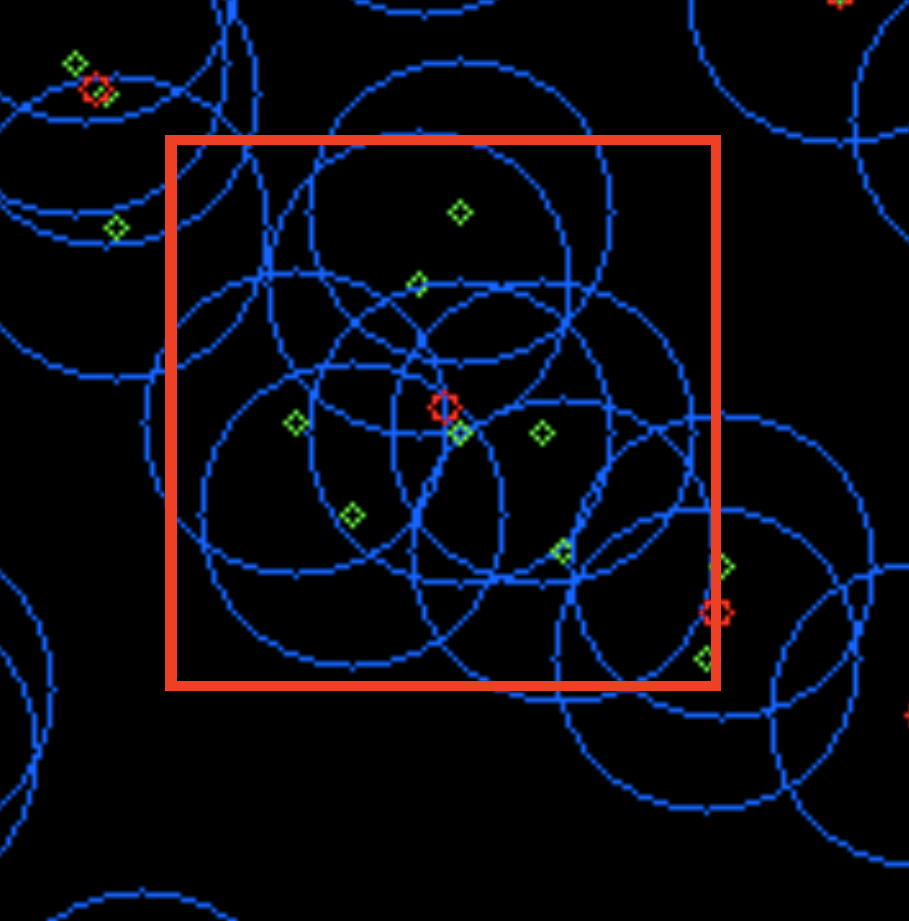
\includegraphics[width=0.3\textwidth]{point_clustering_multiple_spread}\label{fig:point_clustering_multiple_spread}}
	\caption{Different point clustering cases.}
	\label{fig:PointClusteringCases}
\end{figure}

To minimise the group to one single point, which defines the center of the corner, the algorithm uses the average center of all points in the group ~\eqref{eq:PointAverage}.


\begin{equation} \label{eq:PointAverage}
\begin{gathered}
\bar{X} = \sum_{i=1}^{N}X_{i}/N
\\
\bar{Y} = \sum_{i=1}^{N}Y_{i}/N
\end{gathered}
\end{equation}


\subsubsection{Convex hull}
\label{sub:ConvexHull}
Finding the convex hull of a set of points is a good way for this project to find the outer points of our wall that is enclosing the whole building. The convex hull is the smallest convex set of points that contains all points given in a Euclidean space.

The convex hull af a set of points X \begin{equation}conv X \coloneqq \underset{X \subseteq K \subseteq V, K convex}{\bigcap} K  \end{equation} is defined as the intersection of all supersets of X.It can also be described as the set of all limited convex combinations:

\begin{equation}conv X = \{ \sum_{i=1}^{n}\alpha_{i} * x_{i} \mid x_{i} \in X, n \in \mathbb{N}, \sum_{i=1}^{n} \alpha_i = 1, \alpha_i \geq 0  \}]\end{equation}

There are several known algorithms that implement this problems. Examples of those are the Graham-Scan algorithm with a complexity of  $\mathcal{O}(n log n)$ or the Jarvis-March-algorithm with the complexity of $\mathcal{O}(n*k)$ where k is the number of points on the hull itself.

\begin{figure}[h]
	\centering
	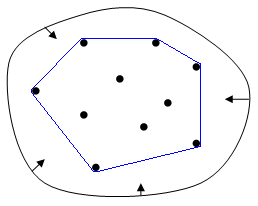
\includegraphics[width=0.4\textwidth]{convex_hull}
	\caption{Example image of a convex hull. The black line around the point-set shows that start of the algorithm as it is closing around all the outer points until  being the convex hull (blue).}
	\label{fig:convex_hull}
\end{figure}


\pagebreak

\subsubsection{Door gap closing algorithm}
\label{sec:DoorGapAlgorithm}

The cascade door training algorithm has found the rectangles that represent the doors. What is needed in the end though is not the door itself but the space in-between the two walls that the door connects. This is so that we can separate the different rooms that have doors in-between.
This algorithm combines the edges that have been found with the Harris-Corner detection and the doors from the cascade door algorithm. It uses a heuristic that works as following. The door algorithm provides four points that mark the edge of the recognized door and build a rectangle.
Added to the rectangle is  a threshold in all directions in which the algorithm searches for edges. The idea is that due to the structure of walls there will be a rectangle made out of four edge points inside the door area that represents the space in-between the walls. It is expected to only find one rectangle, due to the fact that it makes no sense to have a wall go through a door. As well as the fact that there should be no further lines because it it a cleaned up image and any other line except the walls should not be in that image.
To find the rectangle it connects two edges and calculates the angle compared to the x-Axis for all pairs of edges available. Now all the angles get compared to each other. If two edges AB and CD have a similar angle there will be another comparison for the angles between AC and BD or AD and BC. If one of those two is also of a similar we then need to prove that two lines that build a corner have an angle of 90 degree between them. If the opposing lines are all parallel and the angle of one corner is 90 degree we can assume that all other angles have to be 90 degree too and it is therefore a rectangle. 

\begin{figure}[h]
	\centering
	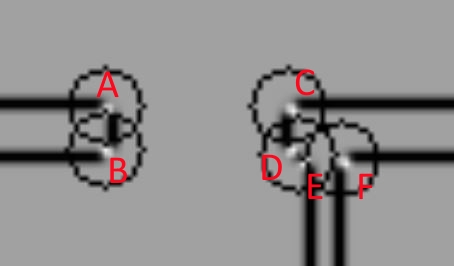
\includegraphics[width=0.4\textwidth]{door_closing}
	\caption{This is an image after being processed by the harris corner detection. All white pixels are part of a corner. The points A,B,C,D will be part of a found door as they create a rectangle. Points E and F will be left out.}
	\label{fig:door_closing}
\end{figure}


\subsection{Structural Analysis}

\subsubsection{ORB algorithm}
\label{sub:ORBAlgorithm}
The algorithm \acrfull{acro:ORB} was used to detect objects in architectural floor plans. It is similar the the to the two other feature matching algorithms like SIFT or SURF. This algorithm is orientation and size invariant which is really important as object size may differ from plan to plan an orientation might even differ within one plan.

The algorithm itself consists out of two algorithms FAST and BRIEF. The FAST algorithm is for finding keypoints in images that match visual features. FAST keypoints are detected with an intensity threshold between a center pixel and the pixels in a circular ring around the center. To select the best keypoints \acrshort{acro:ORB} employs a Harris corner measure (algorithm described in \ref{subsubsec:HarrisCornerDetection}) to find the best $N$ keypoints. Since FAST keypoints have no rotational awareness \acrshort{acro:ORB} introduces the orientation by intensity centroid. The intensity centroid $C$ \eqref{eq:IntesityCentroid}

\begin{equation}\label{eq:IntesityCentroid} C = \begin{pmatrix}
\frac{m_{10}}{m_{00}},\frac{m_{1}}{m_{00}}\end{pmatrix} \end{equation}

is defined by the moments in equation \eqref{eq:MomentsIntesityCentroid}

\begin{equation}\label{eq:MomentsIntesityCentroid} m_{pq} = \sum_{x,y} x^p y^q I(x,y)\end{equation}

To find the orientation $\theta$ \eqref{eq:OrientationORB} the algorithm constructs a vector from the corners center $O$ to the centroid $OC$.

\begin{equation}\label{eq:OrientationORB} \theta = atan2(m_{01},m_10)\end{equation}

Here atan2 is the quadrant aware version of the arcus tangens.

To compare those keypoints to others the algorithm needs the BRIEF descriptor. It does binary test on patches of the image. The binary test $\tau$ \eqref{eq:BinaryTest}is defined by the equation:

\begin{equation}\label{eq:BinaryTest} \tau(p;x,y) := \begin{cases} 1 :p(x) < p(y) \\ 0 :p(x) \geq p(y)\end{cases}\end{equation}

where $p(x)$ is the intensity of $p$ at point x. A feature \eqref{eq:BinaryFeature} to compare the keypoints together is defined as a vector of binary tests: 

\begin{equation}\label{eq:BinaryFeature} f_{n}(p) := \sum_{1 \leq i \leq n}2^{i-1} \tau(p;x,y)\end{equation}

To allow BRIEF to be rotation invariant the descriptor \eqref{eq:BriefDescriptor} will be orientated to the orientation of keypoints. The rotation will be defined by the patch orientation $\theta$ and the rotation matrix $R_{\theta}$ to be $S_{\theta} = R_{\theta}S$.
This orientated BRIEF descriptor is now defined as
\begin{equation}\label{eq:BriefDescriptor} g_{n}(p,\theta) := f_{n}(p)|(x_{i},y_{i}) \in S_{\theta}\end{equation}

By creating a matcher for \acrshort{acro:ORB} that is used by descriptor to compare an image or its features to the features of a target image. If any of those features match the algorithm has likely found the object of the first image in the second image and will return its coordinates \citep{rublee_rabaud_konolige_bradski_2011}.

\subsubsection{Cascade training}
\label{sub:CascadeTraining}
The algorithm used for object detection in this project was first described by Paul Viola in his paper \todo{ACCEPTED CONFERENCE  ON COMPUTER VISION AND PATTERN RECOGNITION 2001 Rapid Object Detection using a Boosted Cascade of Simple Features}. It is based on three key components. One is the "Integral Image" which is an image representation that allows to detect features very quickly. A second component is the learning algorithm "AdaBoost" which select a small number of critical features from a big set. The last component is an algorithm that combines increasingly complex features in a cascade. All of these components provide the basis for a really fast feature detection compared to previously known algorithms.

The object detection for this method is based on features and not pixels. Features can provide additional domain knowledge that would not be know with just pixels. Additionally the detection based on features is processed much faster than a pixel based system. The algorithm uses three different simple features based on the "Haar" basis functions. The value of a two-rectangle feature is the difference of the sum of two regions that are vertically or horizontally adjacent and have the same measurements (see Figure\todo{link figure}). The three-rectangle feature has the same conditions but the value is based on the sum of two outside rectangles and subtracted the sum of a center rectangle. Last is the four-rectangle features which the value is the difference of sums of diagonal pairs of rectangles.
\begin{figure}[H]
	\centering
	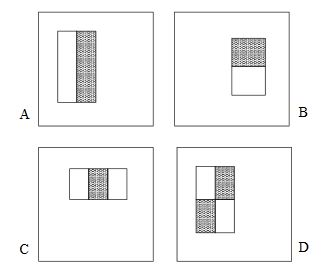
\includegraphics[width=0.4\textwidth]{rectangleFeatures.jpg}
	\caption{Rectangle features in a detection window. There are two-rectangle (A and B), three-rectangle (C) and four-rectangle features in use.}
	\label{fig:rectFeat}
\end{figure}

All features combined are more than 180'000 while the detector has a base resolution of 24x24. This means the rectangle features are overcomplete.
These rectangle features are computed using the representation "integral image". In an integral every pixel is a sum of pixels of the original image that are above and to the left:
\begin{equation}ii(x,y) = \sum_{x'\leq x, y'\leq y} i(x',y')\end{equation}
where ii(x,y) is the integral image and i(x,y) the original. Using two conditions with s(x,y) as the row sum:
\begin{equation}s(x,y) = s(x,y-1)+i(x,y)\end{equation}
\begin{equation}ii(x,y) = ii(x-1,y)+s(x,y)\end{equation}
the whole image can be computed in one pass.
This method helps so we can now compute two-rectangular features from just 6 values instead of having to do all the calculations for the sums each time over whole regions. In addition three-rectangular features only take 8 and four-rectangular only 9 values to calculate its value. This algorithm can only recognize features in vertical, horizontal or diagonal direction due to the nature of our rectangle features.
To train and select a small size of features this algorithm uses the "AdaBoost" method. The basic idea is that there is a feature size over 180'000 features to determine the if an object is recognized or not. The job of this "AdaBoost" is to reduce the amount of features down to a basic set of features that still has a high recognition rate. For each feature the algorithm determines the optimal threshold classification function so that the least amount of examples are misclassified.
To achieve improved detection rate and drastically reduce the computation time this algorithm implements a cascade function. This means that the detection process is that of a degenerate decision tree. A positive result from a classifier triggers the evaluation of the next classifier. If at any point the result is negative the algorithm immediately declares the result as negative and won't be computed any further. The idea is that the first layer rules out a large amount of possibilities with very little computation time. Further stages of the process will reduce further negatives but need additional computation power. The idea behind this process is that in an image most sub-windows will be negative and such should be rejected as early as possible in the cascade process to require fewer computational effort.
The classifier is trained with a training set of positives and negatives. Each stage is trained by adding features until the target detection and false positive rates are met. Stages are added until the overall target for false positive rate and detection rate is met. In the end there is always a balance to between finding high detection rates with low false positive rates and lower time for computation.

\subsubsection{Template Matching}
\label{sub:TemplateMatching}
To find a template $T$ (Figure~\ref{fig:door_template}) in a given image $I$ (Figure~\ref{fig:A_N1_cleaned}), it is possible to use template matching. The algorithm slides the template $T$, pixel by pixel over the original image $I$ and stores the metric of the current pixel, in the correlation image $R$.

There are various kinds of formulas to calculate the matching metric. Usually the formula sums up the matching pixels in the template $T$ and the image $I$ and stores the result as color value, in the correlation image $R$.

\begin{figure}[h!]
	\centering
	\subfloat[Template $T$]{
\includegraphics[width=0.15\textwidth]{door_template}\label{fig:door_template}}
	\hfill
	\subfloat[Image $I$]{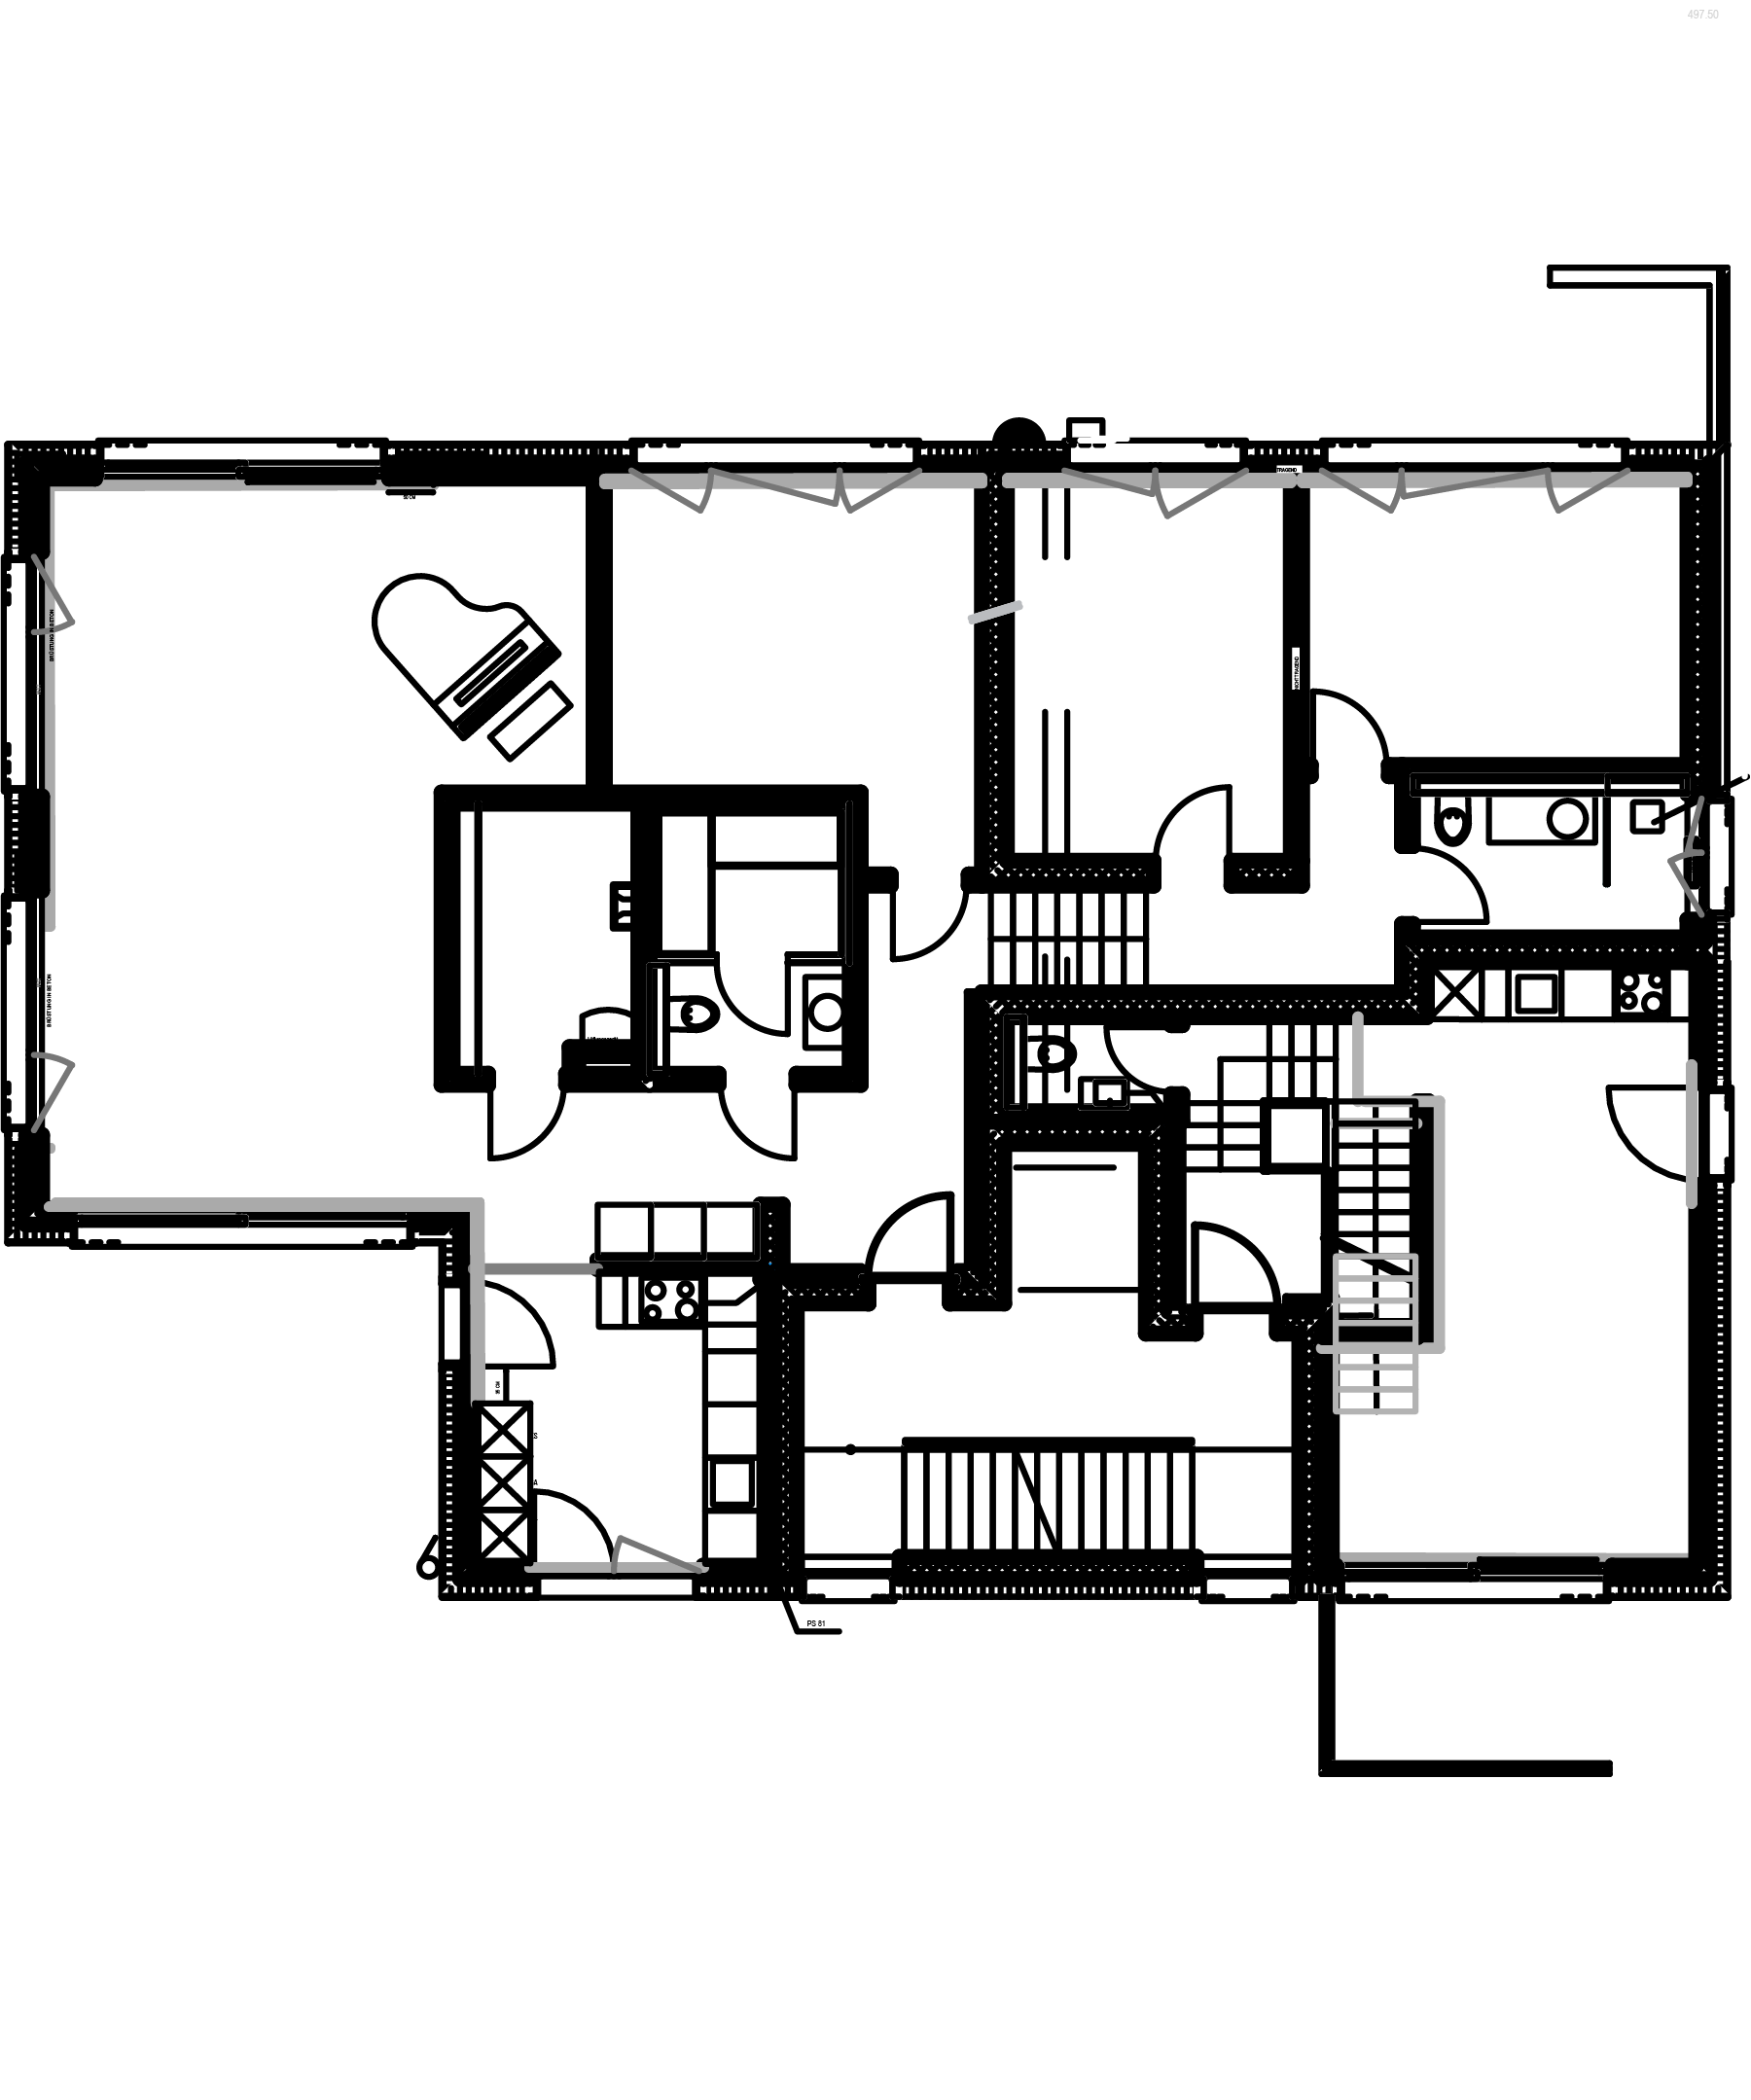
\includegraphics[width=0.4\textwidth]{A_N1_cleaned}\label{fig:A_N1_cleaned}}
	\hfill
	\subfloat[Correlation matrix $R$]{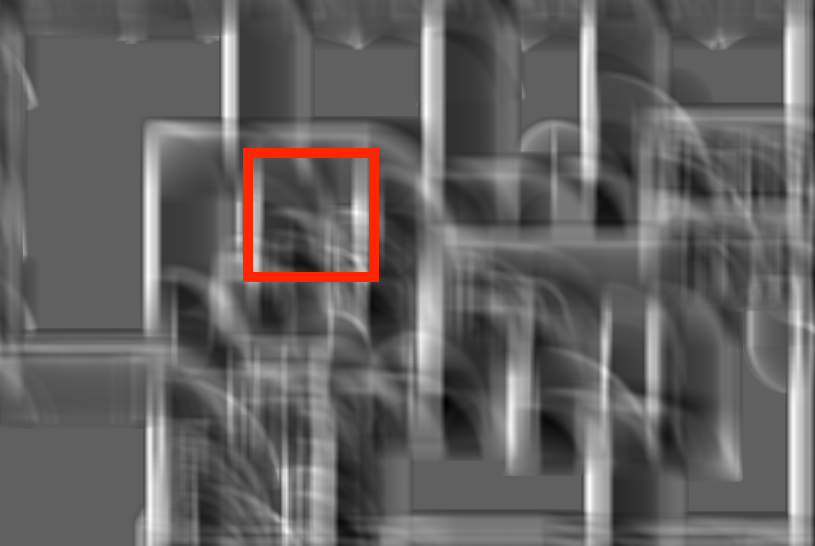
\includegraphics[width=0.4\textwidth]{tm_correlation_matrix}\label{fig:tm_correlation_matrix}}
	\caption{Template matching example. The red rectangle in \ref{fig:tm_correlation_matrix} indicates the brightest location.}
	\label{fig:TemplateMatchingExample}
\end{figure}


The brightest points in the correlation image $R$ (Figure~\ref{fig:tm_correlation_matrix})  indicate the highest matches. If multiple occurances of an object should be detected, it is possible to use a threshold on the correlation matrix $R$ to detect all the correlated locations.

Template matching is a very simple matching method and is not rotation and scale invariant.



 
\subsection{Semantic Analysis}
\subsubsection{Hough transformation}
\label{subsubsec:Hough transformation}
The hough transformation was used as an alternative to the current process to find walls and therefore the rooms. In the implementation it will be explained why this was not implemented in the final project.

The hough transformation is a general approach to find forms like lines or circles in images. This section will discuss how to detect lines in an image.
Any line can be represented as $r = x \cos \theta + y \sin \theta$ which is the "Hessesche Normalenform". The parameter $r$ represents the distance from the origin, in an image the bottom left, to the closest point on a straight line that goes through $(x,y)$. The angle $\theta$ represents the angle between the x-axis and the line we used for our parameter $r$. Any possible straight line that can go through the image can be represented by those parameters. The plane of $(r,\theta)$ is called the Hough space for straight lines.

\begin{figure}[h]
	\centering
	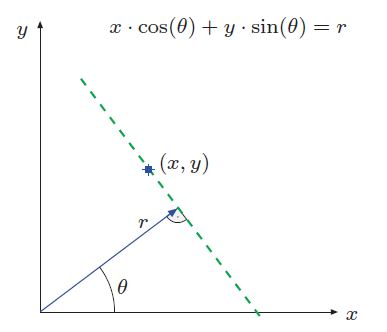
\includegraphics[width=0.4\textwidth]{hough_gerade}
	\caption{This is an example image of a hough-line with the distance $r$ and the angle $\theta$. It represents the hough line $r = x \cos \theta + y \sin \theta$.}
	\label{fig:hough_line}
\end{figure}

The algorithm now uses a two dimensional array called accumulator to detect the existence of a straight line The algorithm now determines for each pixel and its neighborhood if there is a possibility for a line and then increments the value in the accumulator for the representative $(r,\theta)$ values. When done for all pixels on the image, there will be local maxima for $(r,\theta)$ values in the accumulator. Those maxima are the most likely to represent a straight line in the actual image.  

\begin{figure}[h]
	\centering
	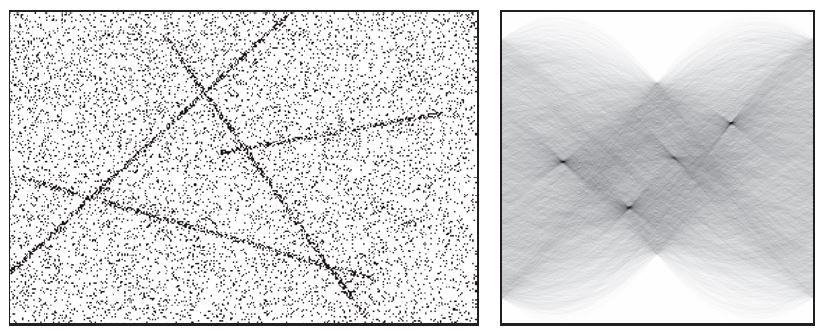
\includegraphics[width=0.4\textwidth]{hough_accumulator}
	\caption{The image on the left side represents an image with lines and some noise on it. The right image represents the Hough plane (accumulator) with local maxima which are highlighted as white pixels.}
	\label{fig:hough_accumulator}
\end{figure}

To find the actual length of the lines there has to be a further algorithm that checks where on those lines that were found the line on the image exists. This can done in several ways and therefore will not be explained here. There are several algorithms described on the internet or for example in the book "Digital image processing: an algorithmic introduction using Java" \cite{burger_burge_2016}.

\pagebreak

\subsubsection{Connected Component Analysis}
\label{sub:ConnectedComponentAnalysis}
Finding connected components is a common way to detect objects in a thresholded image. In this work it is used to detect connected room pixels and calculate the size of each room out of it.

This is accomplished by finding pixels which are adjacent to each other. A pixel is adjacent to another pixel if it is immediate $\mathcal{N}_4$ or $\mathcal{N}_8$ and has the same scalar value. Further the neighbor pixels are labeled with the same label and in the end combined to a region $\mathcal{R}$ \citep[Section 3.3.4]{szeliski_2011}.

\begin{figure}[h]
	\centering
	\subfloat[4-neighbourhood, $\mathcal{N}_4$]{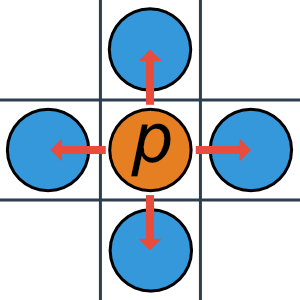
\includegraphics[width=0.3\textwidth]{n4_pixel}\label{fig:n4_pixel}}
	\hfill
	\subfloat[8-neighbourhood, $\mathcal{N}_8$]{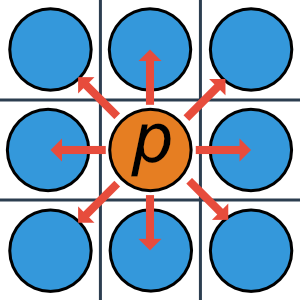
\includegraphics[width=0.3\textwidth]{n8_pixel}\label{fig:n8_pixel}}
	\caption{Pixel neighbourhoods.}
	\label{fig:pixel_neighbourhood}
\end{figure}

The distance $\mathcal{N}_4$ and $\mathcal{N}_8$ refers to the distance between two pixels (Figure~\ref{fig:pixel_neighbourhood}). In $\mathcal{N}_4$ only the four pixels (top, left, bottom, right) are used to determine if two pixels are connected. In $\mathcal{N}_8$ all pixels around the pixel are included into the process \citep{burger_burge_2016}.

For each region $\mathcal{R}$ it is possible to compute statistics like the area (number of pixels) or the perimeter (number of boundary pixels) \citep[Section 3.3.4]{szeliski_2011}. These statistics are used for example to determine the actual room size.

\subsubsection{Watershed}
\label{subsub:watershed}
The watershed-algorithm in our project is used for segmentation of the different rooms. It can find rooms indifferent of its shape.
\\
The algorithm is processed on a gray-scale image on which the color intensity is analogous to the height in a height map. The watershed in use does flooding. The idea is to place a water source in each regional minimum and flood the entire relief. It will stop if it meets a different water source or an impassable barrier.

The basic algorithm uses three different markings for all regions. The values I for each region can be:
\begin{equation}I(u,v) = \begin{cases} 0 & background \\  255 & foreground \\ 1..254 & regions \end{cases} \end{equation}

It is a really simple algorithm where it starts with looking for an unmarked foreground pixel. All pixels of the region that are connected to this starting pixel will be visited and marked. There are three different ways to do this process. It can be a recursive, an iterative depth-first or breadth-first flood filling. It is not clear what implementation OpenCv uses. In the end all of the methods lead to a similar result and thus will not be discussed further. 


\section{Result}
This section covers the results of this project. It will explain, how the final workflow works and what kind of product were produced during the time of this bachelor thesis.

\subsection{Discussion}
\label{sub:Discussion}
In this section we will discuss all the results shown in the implementation. It will highlight the algorithms used and then conclude with a comparison of our results to the other works mentioned "Introduction" under "Similar works".

The machine learning approach, called "Cascade classifier", for door detection shows good results. Most doors on the floor plans can be detected. On all plans the F1-Score was at least at 75 percent. This was good enough for a good implementation of the gap closing algorithm. Another important notice is, that cleaned floor plans show an improvement in detection rate of the F1-score up to a 100 percent. This shows that with little effort the detection can work at very high rates. All of these results can be found in figure~\ref{fig:CCF1ScoreGraph}. What is also shown with this graph is, that the detection rate can be further improved if better or more training images can be found. Almost every training we did showed improvements and with more time it is likely to create a better cascade file and let this trend continue.

The door closing algorithm based on the door detection algorithm shows very good results as well. As seen in figure~\ref{fig:simpleDoorClosing}, the door closing algorithm works in most cases very well. The F1-Score is for all but one image above 75 percent. Very important here is the Recall, it is on more than half of the images at a 100 percent. This means that all doors on the plan are closed. The low precision is due to the fact that some windows are also recognized as doors, therefore the plan has quite a few false positives. It is important to remark, that this algorithm handles false positives very well. In most cases the detection of a false positive will not lead to a negative effect, as it just draws over a wall. A further description of this problem is found in section~\ref{sec:DoorClosingComparison}.

The room detection done based on all this preprocessing, shows results above 80 percent for the F1-Score on all of the cleaned up plans. As explained in section~\ref{sec:ConnectedComponents}, the uncleaned versions have problem with the outer wall closing and most of them show terrible results with room detection. All of these results are based on the fact, that no post processing from the user was done. The exact values can be found in figure~\ref{fig:RoomDDResult}. What improved the room detection by a lot was the user interaction as show in figure~\ref{fig:RoomDDEResult}. On all plans, the F1-Score is above 80 percent, most of them are even on a 100 percent. With enough user interaction, all scores can be on a 100 percent, as the user can basically fully redraw the floor plan to an optimal one for detection. This graph represents tests with user interaction. The time used is comparable to that what user a user would take if the program would be used in a working environment.

Compared to the works of Mace, Valveny,Loctea and Tabbone \citep{mace_valveny_loctea_tabbone_2010} and Ahmed,Liwicki,Weber and Dengel \citep{ahmed_liwicki_weber_dengel_2012}, this work shows some improvement. Our algorithm shows an average of 83.8 percent of room detection accuracy on cleaned up plans. This is slightly above the 82 percent that Ahmed,Liwicki,Weber and Dengel showed. It is an bigger improvement if you compare it to their 79 percent, which was the same algorithm but without combining rooms based on room labels. It is a big step compared to the 69 percent detection accuracy achieved by Mace, Valveny,Loctea and Tabbone. Generally can be said, that uncleaned floor plans will achieve a detection accuracy still below 40 percent, as there is just too much noise that can not be canceled. But simple floor plans or little pre-cleaning can boost the detection rate of those algorithms in the higher 90 percent without additional user input. 

The comparison in figures \ref{fig:ClicksPerPlan} and \ref{fig:TimePerPlan} show the improvement that the automated algorithm shows compared to what is used at the PlanfabrikGmbH. The graphs show that the time and clicks used for analyzing the plans with the algorithm show about the same no matter how big or complicated the plan is. This is contrary to the current approach, which takes more time and clicks with more difficult plans. Generally can be said that time and clicks used are less when using the new algorithm. But the time and effort saved is better the more complicated a plan is. 

\subsection{Workflow}
During the time of this project, we tried out different algorithms and processes (Section~\ref{sub:Discussion}), to create a workflow, which solves the stated task (Section~\ref{sub:ProblemDescription}).

\begin{figure}[H]
	\centering
	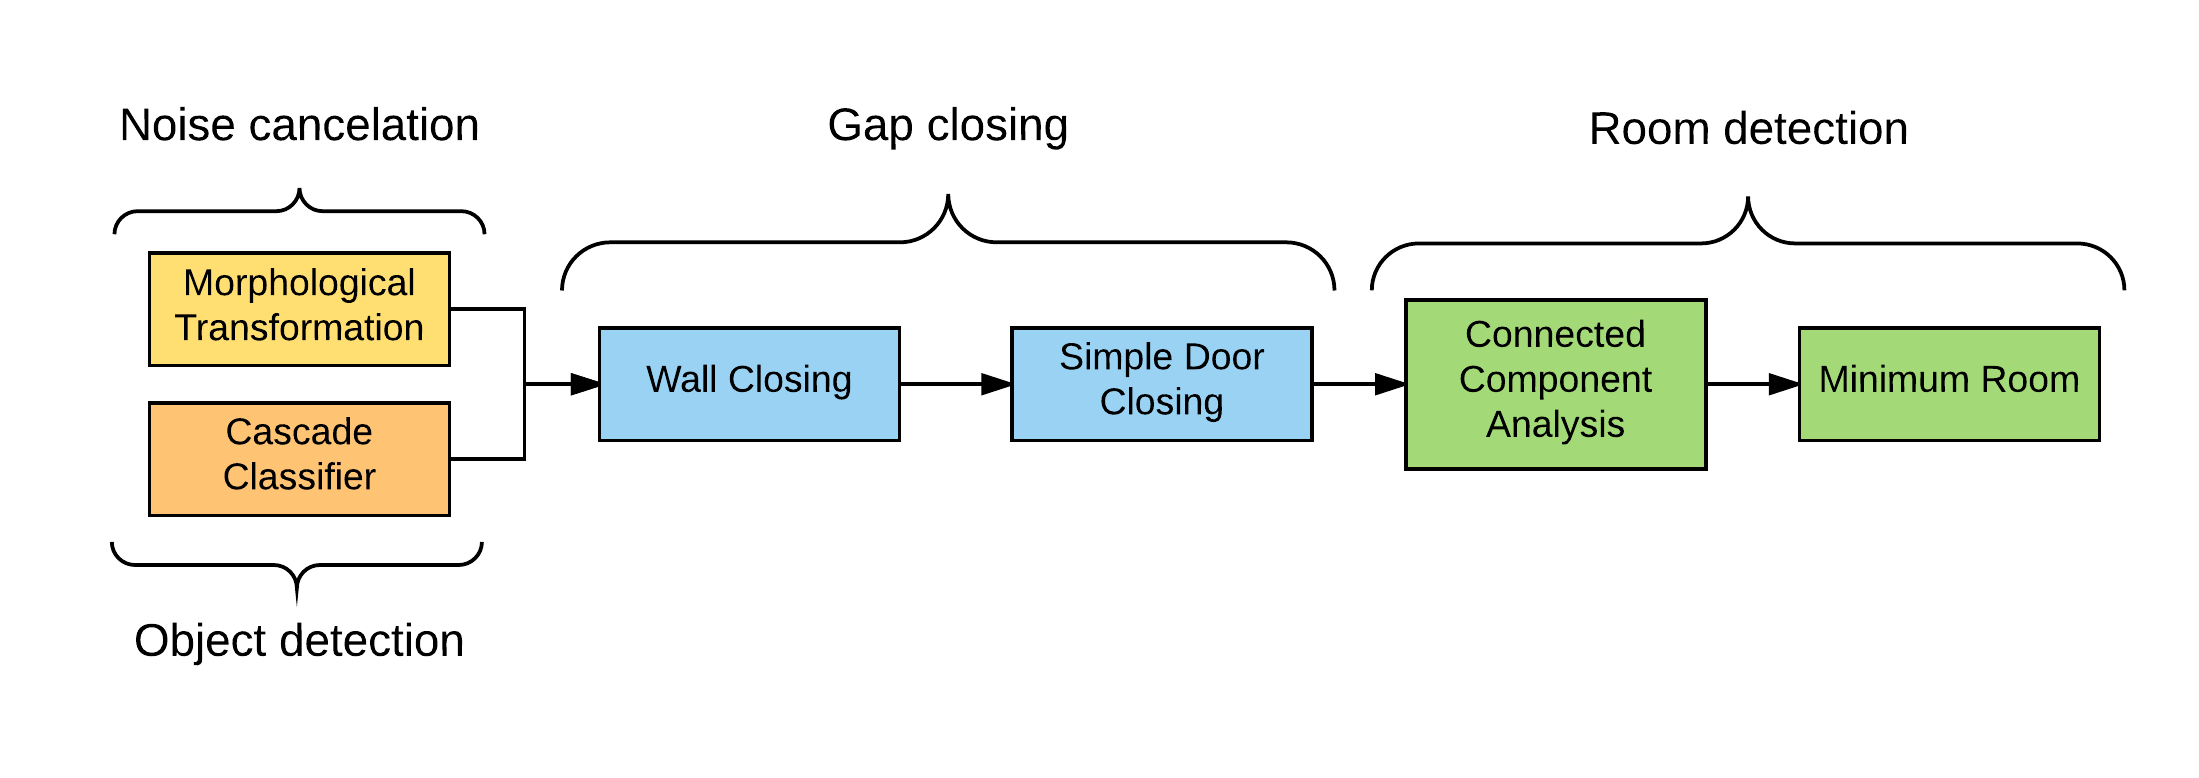
\includegraphics[width=1.0\textwidth]{FinalWorkflow}
	\caption{Final workflow flowchart.}
	\label{fig:FinalWorkflow}
\end{figure}

The workflow is visualised in figure~\ref{fig:FinalWorkflow} is the same workflow as the workflow three, described in section~\ref{sub:workflow3}.

It starts with the object detection (Section~\ref{sub:ObjectDetection}), which detects all doors on a floor plan. This information is saved into the meta image format (Section~\ref{sub:MetaFormat}) for further processing. Then the noise cancelation (Section~\ref{sub:NoiseRemoval}) removes noise like furniture, markings and other elements on the plan, to create a skeleton of the building walls.

Due the fact, that the noise cancelation removes also the windows of the building, the wall closing algorithm (Section~\ref{sub:WallClosing}) finds the outer contour and closes the gaps. Together with the information gathered in the objection detection step, the simple door closing algorithm (Section~\ref{sub:SimpleDoorClosing}) closes the gaps between the walls, where the doors should be.

After the cleanup and reconstruction process, the room detection is processed (Section~\ref{sub:RoomDetection}). As final step, the minimum room detection (Section~\ref{sub:MinimumRoom}) filters out rooms, which are too small, in relation to the average room size.


\subsection{Prototype}

\subsection{Limitations and restrictions}
\section{Conclusion}
\subsection{Extensions}
In this topic we discuss what additional measures can be taken to improve and extend this program. It will also show what the preparations were to provide an easy implementation for future extensions.

\subsubsection{Object detection}
\label{sub:FutureObjectDetection}
As of now, only doors are being matched with the cascade classifier. There are several objects that could further be identified. Those objects are showers, toilets, baths, windows and different sorts of closets.
There was a try to identify windows with the cascade classifier already. But for the case of windows it is near impossible to find a good classifier. Most of the plans provided have a different structure or a different symbol and sometimes they are even marked differently within the same plan. But with the other objects this should be possible. Those objects would help remove noise on the initial plan as they would be removed after their detection. Additionally these object define different zones as described in section~\ref{sub:ZoneDetection}. To provide a head start for future work on this project,there are trained cascade files for each of those objects. Additionally the class that implements the cascade classifier in this project can reference a cascade file and discover the object trained. Therefore all steps to detect the objects are already provided. It is the implementation in a workflow and the usage to define zones that are not yet implemented and need work. In our opinion, implementing this additional detection will make detecting the walls easier as there is less noise and it will improve the room detection as a direct result of that.

\subsubsection{Zone detection}
\label{sub:RoomZones}
\label{sub:ZoneDetection}
The zone detection was originally one of the goals of this project. As there was not enough time, we provided a lot of work to make it easily implementable for a future project. As described in the object detection~\ref{sub:FutureObjectDetection}, these zones are defined by different objects.
There are three different zones:
\begin{table}[h]
	\centering
	\label{tab:Zones}
	\begin{tabular}{@{}lll@{}}
		"Blindflächen" & This zone consists out of the elements showers, baths and small \\
		& walls that are an extension to the real wall.\\
		"Randzonen" &  This zone is connected to all windows on the outside of a house. \\
		"Stellflächen" & This zone consists of kitchen combinations and closets.\\
	\end{tabular}
\end{table}	

The reason different zones exist are that there will be different density of heating tubes or none at all under those different zones. The idea is, that each room is split into these zones and the zones are returned in addition to the room polygon. The big problem with this addition is, that windows are difficult to detect and therefore the "Randzone" is hard to detect without a heuristic. The current solution to window closing~\ref{sub:WallClosing} could be extended to find empty spaces inbetween the walls and then define the gaps as their location. This can be a solution but it is prone to difficult structures on the outside wall (like balcony's etc.) and special constructs in the outer walls. Basically even a big white space in a wall could possibly result in a gap and would then be recognized as a window. Therefore if there is a possibility to standardize the symbol for a window and then detect it with our cascade classifier. This detection would be a lot smoother.

\subsubsection{3D-plan}
An idea, that was mentioned by the PlanfabrikGmbH at the start of the project was, that with object detection 2D-plans could automatically transformed into 3D-plans. This idea could be implemented with some elements used in this work. Specifically the object detection could be used to detect all elements that are available on the floor plans. When recognized, a 3D-plan could be created with some additional information about the size of these objects. The challenge with this problem will be, that there is no standardization for objects like walls or any other within a floor plan itself. Therefore it is very unlikely that an automated detection would work within this environment. A good 3D-plan creation will first need a guideline of how object symbols are to be drawn and architects would have to follow it.


\subsection{Acknowledgment}
We would like to thank both the Planfabrik GmbH and the Fachhochschule Nordwestschweiz for the possibility to work on such an interesting problem. In specific we would like to thank Oliver and Patrick Stalder for their great support and their insight provided into their work. They both were very supportive and always very interested which made them a pleasure to work with! Additionally we would like to thank Prof. Dr. Simon Schubiger as our coach, for his coaching and all the ideas we were able to discuss. We are very thankful for his continued support and all of his advice!
\section{Annex}

\subsection{Figures}
\begin{table}[H]
\small
\centering
\caption{DWG / DXF evaluation matrix.}
\label{tbl:DWGEvaluationMatrix}
\makebox[\linewidth]{
\begin{tabular}{@{}llllllll@{}}
\toprule
Name & Vendor & Price & Last Update & License & Read & Write & Comment \\ \midrule
YCAD & Ed Karlo & - & Aug 07, 2015 & LGPLv2 & Yes & ? & \begin{tabular}[c]{@{}l@{}}confusing \& \\ no documentation.\end{tabular} \\
Teigha & ODA & 2000 USD/Y & - & Commercial & Yes & Yes &  \\
Kabeja & - & - & Mar 12, 2008 & Apache-2.0 & Yes & No &  \\
Tika & Apache & - & Oct 19, 2016 & Apache-2.0 & Yes* & No & *Meta text reader. \\
jnetcad & J. Raida & ? & Apr 28, 2016 & Commercial & Yes* & Yes* & \begin{tabular}[c]{@{}l@{}}*Only converter \\ for 3D Objects.\end{tabular} \\
CaffViewer & DeCaff & 1350 Euro & May 17, 2016 & Freeware & Yes & Yes &  \\ \bottomrule
\end{tabular}
}
\end{table}

\subsection{Developer Guide}
This section describes, how to extend the application developed in this work. It is split into different tasks, which will most likely be done in the future.

\subsubsection{Installation}
The software is still a prototype and not packaged into an executable. To run the software, you have to run the \texttt{run.sh} (Unix) or \texttt{run.bat} / \texttt{run64.bat}  (Windows).

\subsubsection{Development prerequisites}
For development on the existing project, you have to install the JDK 8 (Java Development Kit). The download link to the JDK is the following:

http://www.oracle.com/technetwork/java/javase/downloads/jdk8-downloads-2133151.html

The project itself can be built with the \textit{gradle build tool} (https://gradle.org/) (Listing~\ref{lst:GradleBuild}).

\begin{lstlisting}[caption={Gradle build tool build of the project.}, label={lst:GradleBuild}, language=Kotlin]
// unix
gradlew build

// windows
gradle.bat build
\end{lstlisting}

\subsubsection{Adding new algorithm}
To add a new algorithm you have to create a new class, which implements the \textit{IAlgorithm} interface. The interface and algorithms are described in section~\ref{sub:algorithm}, but we will give you here a short overview over the interface and how to implement it.

We recommend, to split up different parts of a new process into different algorithms, which enhances the maintainability of an algorithm.

\begin{figure}[H]
  \centering
      \includegraphics[width=0.6\textwidth]{IAlgorithm_CD}
  \caption{Algorithm interface class diagram.}
  \label{fig:IAlgorithm_CD_DG}
\end{figure}

In figure~\ref{fig:IAlgorithm_CD_DG} you see the methods, which have to be implemented to run the algorithm. The very basic version of an algorithm just returns the input image as it is (Listing \ref{lst:basicAlgorithm}).

\begin{lstlisting}[caption={Basic version of an algorithm.}, label={lst:basicAlgorithm}, language=Kotlin]
class MyAlgorithm : IAlgorithm
{
    override val name: String
        get() = "MyAlgorithm"

    override fun run(image: AFImage, history: MutableList<AFImage>): AFImage {
        return image
    }
}
\end{lstlisting}

If you change the original image, it makes sense to create a copy of the incoming image, because the algorithm will maybe run multiple times. There are multiple ways to copy a \textit{Mat}, but we have provided an extension method called \textit{copy()} (Listing~\ref{lst:extendedAlgorithm}, Line~\ref{line:AlgorithmCopy}), which creates a deep copy of the image.

If your algorithm uses parameters, which should be possible to change by the user, you can flag the parameter variables with an \textit{AlgorithmParameter} attribute (Listing~\ref{lst:extendedAlgorithm}, Line~\ref{line:AlgorithmParameter}). You then also have the possibility to set the range of the parameter and provide a short help text (Listing~\ref{lst:extendedAlgorithm}, Line~\ref{line:AlgorithmHelpText}). These informations will be read by the parameter window and shown during the process.

\begin{lstlisting}[caption={Extended version of an algorithm.}, label={lst:extendedAlgorithm}, language=Kotlin, escapechar=$]
class MyAlgorithm : IAlgorithm
{
    @AlgorithmParameter(name = "Threshold",
            minValue = 0.0,
            maxValue = 255.0,
            majorTick = 1.0,
            helpText = "Set the threshold value!") $\label{line:AlgorithmHelpText}$
    var threshold = 128.0 $\label{line:AlgorithmParameter}$

    override val name: String
        get() = "MyAlgorithm"

    override fun run(image: AFImage, history: MutableList<AFImage>): AFImage {
        val img = image.image.copy() $\label{line:AlgorithmCopy}$
        
        // do image processing
        img.threshold(threshold)

        history.add(AFImage(image.image, "Image before threshold")) $\label{line:AlgorithmHistory}$
        return AFImage(img, "Result")
    }
}
\end{lstlisting}

To provide images to the user from between the algorithm, you just have to add the image to the \textit{history} list (Listing~\ref{lst:extendedAlgorithm}, Line~\ref{line:AlgorithmHistory}). The images provided in there are shown in the parameter window (Section~\ref{sub:parameter_window}).

\subsubsection{Extending the user interface}

To edit the user interface, you have to edit the \textit{MainWindow} controller class. In this section we will explain how to add a new button to the user interface, to export the current displayed image.

The user interface is written with the UI Framework JavaFX 2 and uses FXML files to define the layout of the different forms. We recommend to use the SceneBuilder application from Gluon to edit these layout files (http://gluonhq.com/products/scene-builder/).

For more information about the user interface, have a look at the section~\ref{sub:userInterface}.

\begin{figure}[H]
	\centering
	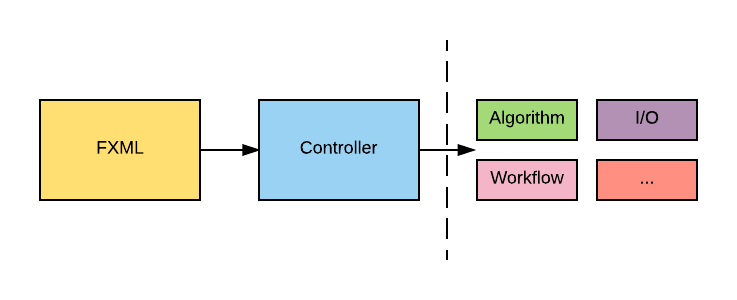
\includegraphics[width=0.8\textwidth]{fxmlArchitecture}
	\caption{User interface architecture.}
	\label{fig:fxmlArchitecture}
\end{figure}

As seen on figure~\ref{fig:fxmlArchitecture}, the user interface is split into two parts. The first one is called FXML and defines the layout of the interface. The second one is the controller, which defines the actions and events, which can happen on the interface. For example, for the \textit{MainWindow} there is a \textit{MainWindow.fxml} and a \textit{MainWindow.kt} file in the source code.

\begin{lstlisting}[caption={MainWindow.fxml with new button.}, label={lst:fxmlwithbutton}, language=XML, escapechar=$]
    <Separator orientation="VERTICAL" />
    <Button onAction="#exportLayer" text="Export SVG" />
    <Button onAction="#exportToCSV" text="Export CSV" />
    <Button onAction="#saveImage" text="Save Image" /> $\label{line:fxmlSaveImage}$
</children>
\end{lstlisting}

First of all, you have to add the extra button to the layout. In listing~\ref{lst:fxmlwithbutton} on line~\ref{line:fxmlSaveImage} there is the new button defined. The \textit{onAction} attribute is a link to a method in the controller of the view.

Now, you have to implement the behaviour of the button on the controller side. There you have to create a function, which is called like the \textit{onAction} attribute value.

\begin{lstlisting}[caption={Save image controller code.}, label={lst:saveImage}, language=Kotlin, escapechar=$]
fun saveImage(e : ActionEvent)
{
    val stage = (e.source as Node).scene.window as Stage

    val fileChooser = FileChooser()
    fileChooser.initialFileName = "image.png"
    fileChooser.title = "Export image as png"
    fileChooser.extensionFilters.addAll(
            FileChooser.ExtensionFilter("PNG", "*.png"))

    val file = fileChooser.showSaveDialog(stage)

    if (file != null) {
        val writableImage = WritableImage(canvas.canvas.width.toInt(),
                canvas.canvas.height.toInt())
        canvas.canvas.snapshot(null, writableImage)
        val renderedImage = SwingFXUtils.fromFXImage(writableImage, null)
        ImageIO.write(renderedImage, "png", file)
    }
}
\end{lstlisting}

First, you have to show a file chooser, where the user is able to choose the file output location. To save the current image, you have to copy the canvas element into a writable image.

\subsubsection{Training new classifiers}

The objection detection in this project is primarily achieved with cascade classifiers (Section~\ref{sub:CascadeTraining}). This section gives a brief overview, how to train new objects with cascading classifiers and how to add it to the current process.

To train a new object, you should have following prerequisites:

\renewcommand{\labelenumi}{\alph{enumi})}
\begin{enumerate}
    \item Minimum 25 images of the object to detect (positives).
    \item Minimum 50 large images of the background (negatives).
    \item OpenCV installed (http://opencv.org/).
    \item ImageMagick installed (https://www.imagemagick.org/).
    \item OpenCV Sample Annotator installed (https://github.com/cansik/opencv-sample-annotator).
\end{enumerate}

\paragraph{Setup new training project}

The source code of this project contains a folder called \textit{/training}, which contains a shell script called \textit{train.sh}. This shell script is there to train a new classifier, but it needs some files at the right place to run.

The folder also contains an example directory structure called \textit{/training/example}. We recommend to copy this structure, rename it to the object, you want to recognise (for example \textit{doors}) and add your positive images to the \textit{positive} folder and the negative images to the \textit{negative} folder.

\paragraph{Annotate positive images}

Now you have to annotate your positive files, which means that you have to select the object in your positive images. We have developed a simple application (Figure~\ref{fig:SampleAnnotator}), which helps you to annotate the images.

\begin{figure}[H]
	\centering
	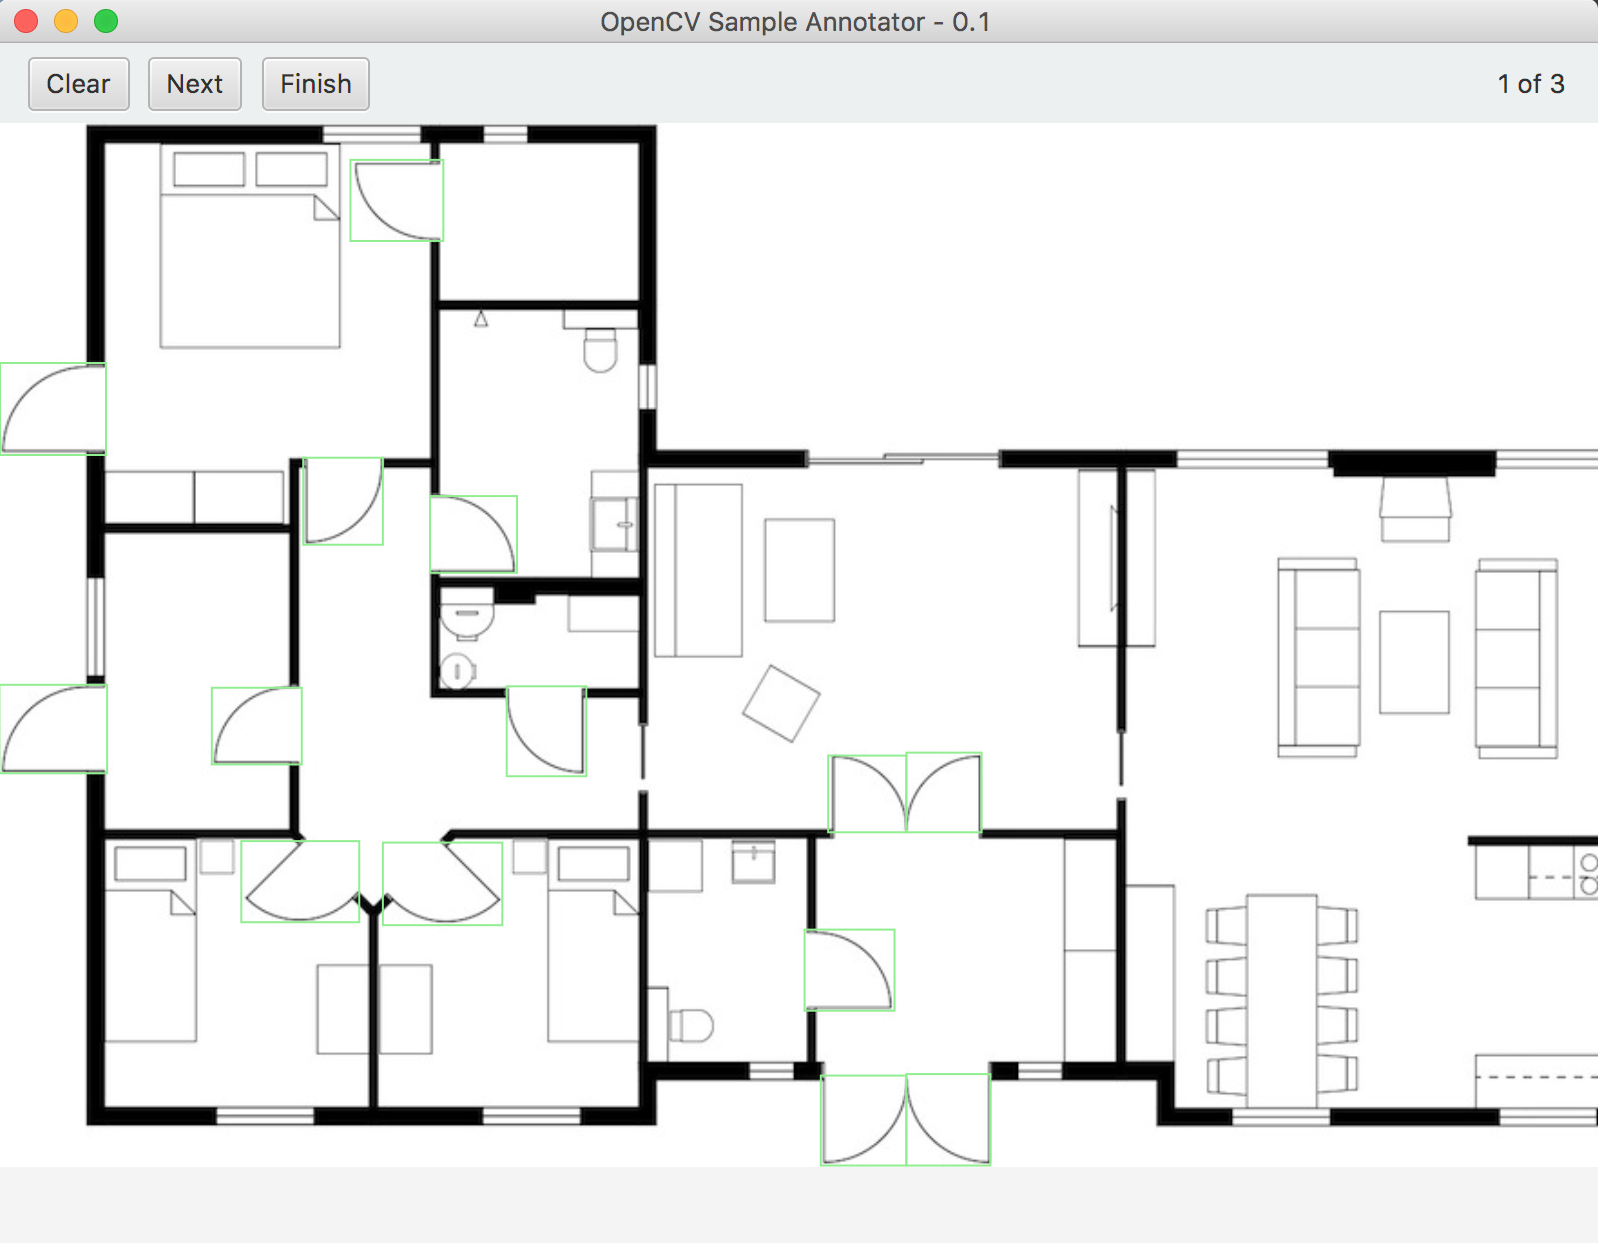
\includegraphics[width=0.8\textwidth]{SampleAnnotator}
	\caption{OpenCV Sample Annotator.}
	\label{fig:SampleAnnotator}
\end{figure}

If you start the application, you have to select the dataset. These are your positive images, which are stored in the \textit{positive} folder. The second thing to select, is the output file. You should store it directly into the project folder (\textit{/training/doors}) as \textit{positives.txt}.

Then you have to draw a rectangle around every object, that occurs in the image. If you have annotated all objects, click next and annotate the next image until you are finished. The application automatically saves the annotated regions into the \textit{positives.txt} file.


\paragraph{Process negative images}
If you have just 50 negative images, you should process these images first and create cropped versions of it, which helps to get better training results \citep{ball}. We recommend to gather large negative images and then split the images into smaller parts.

This can be done with \textit{ImageMagick} batch processing. Navigate into your \textit{negative} folder and run following command of listing~\ref{lst:ImageCropping}.

\begin{lstlisting}[caption={Image cropping.}, label={lst:ImageCropping}, language=Kotlin, escapechar=$]
convert -crop 10%x10% +repage image.jpg image_part_%d.jpg
\end{lstlisting}

\paragraph{Start training}
Now all preprocessing steps are finished and you finally can start the training of your new object. The training process is started by running the script \textit{train.sh} with following attributes:

\begin{enumerate}
    \item \textit{PROJECT}: The name of your project folder.
    \item \textit{WIDTH}: The width of your positive objects.
    \item \textit{HEIGHT}: The height of your positive objects.
    \item \textit{NUMPOS}: The number of annotated positive objects.
    \item \textit{NUMNEG}: The number of negative images.
\end{enumerate}

We recommend a small \textit{WIDTH} and \textit{HEIGHT}, because the training process is faster and you are abel to detect smaller objects. In listing~\ref{lst:RunTraining} you see an example how to run the training.

\begin{lstlisting}[caption={Run training.}, label={lst:RunTraining}, language=Kotlin, escapechar=$]
./train.sh doors 14 14 10 200
\end{lstlisting}

\paragraph{Add trained classifier to algorithm}
When the training is finished, you will find the \textit{cascade.xml} in your project folder in the directory \textit{trained}. This file contains the trained data and is used by the algorithm to run the detection.

To add this file to the existing process, you have to add it into the \textit{cascade-files} folder and add a new classifier detector algorithm, to the default workflow (Listing~\ref{lst:CCDefaultWorkflow}).

\begin{lstlisting}[caption={New classifier in default worfklow.}, label={lst:CCDefaultWorkflow}, language=Kotlin, escapechar=$]
val defaultWorkflow = Workflow(
        arrayListOf(
                CascadeClassifierDetector("cascade.xml", "doors"),
                MorphologicalTransform(),
                ExteriorWallClosing(),
\end{lstlisting}
\bibliography{quotations}
\section{Declaration of Academic Integrity}
Hereby, we declare that we have composed the presented paper independently on my own and without any other resources than the ones indicated. All thoughts taken directly or indirectly from external sources are properly denoted as such. This paper has neither been previously submitted to another authority nor has it been published yet.
\vspace{0.3in}
\Signatures{Florian Bruggisser}{Alexander Wyss}

\clearpage
\printglossary

\clearpage
\listoffigures

\end{document}